\chapter{Обработка сигналов со сцинтилляционных детекторов с разделением наложенных импульсов}
\label{ch:ch2}

% ==========================================================

\section{Проблемы обработки сигнала сцинтилляционных детекторов}

При регистрации гамма кванта веществом сцинтиллятора происходит вспышка света, которая с помощью ФЭУ может быть преобразована в электрический сигнал с амплитудой, прямо пропорциональной поглощённой сцинтиллятором энергии. Для кристаллов NaI, LaBr3(Ce), BGO, и др. форма импульса детектора зависит от характеристик кристалла и светоприёмника, и не меняется в зависимости от энергии поглощённого гамма кванта \cite{Gin2008}. Также форма импульса их может меняться при изменении температуры, напряжения смещения или загрузки \cite{Renker2009,Grodzicka2015}. При регистрации нейтронов органическими сцинтилляторами импульсы, вызванные протонами отдачи, отличаются по форме.  Обработка таких сигналов, особенно в присутствии высокого гамма-фона, является отдельной задачей (которая тоже может быть решена с использованием модифицированных методов, описанных в настоящей главе, однако этот вопрос выходит за пределы темы настоящей работы \cite{Iliasova2020}), поэтому мы ограничиваемся рассмотрением обработки сигналов гамма-детекторов. 

Сигнал с детектора может быть записан с помощью АЦП и проанализирован во время измерения, либо после его окончания. Одна из основных проблем получения спектра при большой загрузке заключается в том, что большое число импульсов, генерируемых гамма квантами при поглощении веществом сцинтиллятора, оказываются наложенными друг на друга. Доля наложенных импульсов зависит от времени высвечивания сцинтилляционного кристалла и от числа регистрируемых сигналов в единицу времени (загрузки детектора). Таким образом, выбор кристалла с меньшим временем высвечивания и использование высокоскоростного АЦП позволяет уменьшить число таких импульсов. С другой стороны, можно проводить дополнительную цифровую обработку сигнала, измеряемого на выходе спектрометрического тракта, с целью получения информации о событиях, сигналы которых оказались наложены друг на друга. А комбинация <<быстрого>> кристалла и алгоритмов цифровой обработки совместно позволяет ещё более увеличить максимальную скорость счёта детектора, при которой возможна работа диагностики токамака.

В настоящей работе описано два алгоритма, которые могут быть применены для цифровой обработки сигнала сцинтилляционного гамма-детектора в условиях регистрации с большим числом наложенных импульсов. Первый из них --- метод фиттинга, является модификацией разработанного в нашей группе метода \cite{Gin2008}. Второй --- метод деконволюции, который так же является нашей оригинальной разработкой в применении к осциллограммам. Проведено сравнение этих алгоритмов как между собой, так и с двумя тривиальными алгоритмами обработки осциллограмм (по максимуму и по сумме под пиком) в применении для обработки как модельных сигналов, так и измеренных сигналов.

Все описанные алгоритмы реализованы как часть компьютерного кода DeGaSum, разработанного автором, который так же позволяет обрабатывать спектры гамма излучения и на их основе получать функции распределения убегающих электронов и быстрых ионов \cite{Khilkevitch2020}.

% ==========================================================

\section{Генерация модельного сигнала}
\label{sec:SignalGeneration}

Для тестирования и изучения характеристик алгоритмов анализа амплитуды импульсов мы смоделировали форму сигнала с детектора (осциллограммы) с известным количеством событий с известными амплитудами. Сгенерированная осциллограмма может быть описана следующей формулой:
\begin{equation}
  \label{eq:OscShapeBase}
  s(t) = z(t) + n(t) + \sum\limits_{j = 0}^{L} A_j p(t-t_j)
\end{equation}
где $t$ --- время, $s(t)$ --- измеряемый сигнал, $z(t)$ --- нулевая линия (постоянная или меняющаяся во времени медленно по сравнению с длиной испульса от события регистрации гамма кванта), $n(t)$ --- шум, $L$ --- число зарегистрированных событий, $A_j$ и $t_j$ --- амплитуда и время события регистрации гамма кванта, $p(t)$ --- форма импульса, которая регистрируется при попадании гамма кванта в детектор. 

Для записи сигнала обычно используется <<быстрое>> АЦП с частотой регистрации намного болше, чем характерные времена роста и спада импульа (например, для детекторов на основе кристаллов NaI(Ti) можно использовать АЦП с частотой 30~МГц \cite{Shevelev2004}, для детекторов на основе LaBr3(Ce) испоьзуются АЦП с частотой 250~МГц \cite{Shevelev2014,Shevelev2018,Khilkevitch2020}). Далее предполагается, что время указано в отсчетах АЦП. Поскольку АЦП измеряют сигналы дискретно, используется дискретная форма выражения~\ref{eq:OscShapeBase}:
\begin{equation*}
  s_i = z_i + n_i + \sum\limits_{j = 0}^{L} A_j p(i-t_j)
\end{equation*}
где $i$ --- номер отсчёта АЦП ($ t_i \equiv i $).

Шумовая составляющая сигнала обусловлена как собственным шумом АЦП, так и внешними причинами (наводки от внешних устройсв, шумы детектора, и т.п.). Значения шума в различные моменты времени считаются независимыми. Для моделирования мы предполагаем, что $n(t) = R^g( \sigma_n )$, где $R^g(\sigma_n)$ --- случайное число с гауссовым распределением со средним значением, равным 0, и стандартным отклонением, равным $\sigma_n$.

Форма импульса $p(t)$ зависит от материала сцинтиллятора и размера кристалла, высоковольтного смещения ФЭУ, характеристик детектора, спектрометрического тракта и частоты дискретизации АЦП. Форма импульса не зависит от времени и амплитуды регистрации события. Предполагается, что $\lim_{t \to \pm \infty} p(t) = 0$ и $\max_{t} | p(t)| = 1$. Форму импульса, вызванного гамма-квантом в сцинтилляционном детекторе, можно аппроксимировать следующей аналитической формулой \cite{Gin2008,Shevelev2004,Shevelev2016,Khilkevitch2020}:
\begin{equation}
  \label{eq:PulseShape}
  p(t) = \begin{cases} 
    t > 0   & P_n \left( 1 - e^{-t/t1} \right)^k \cdot \left( e^{-t/t2} + B e^{-t/t3} \right) \\ 
            t \le 0 & 0
         \end{cases}
\end{equation}
где $P_n$ --- нормировочный коэффициент, $t_1$, $t_2$, $t_3$, $B$, $k$ --- численные параметры импульса, зависящие от характеристик кристалла и светоприемника. В некоторых случаях лучше описывает форму импульса иное выражение \cite{Khilkevitch2020}: 
\begin{equation*}
  p(t) = P_n \cdot \frac{1}{ \left( 1 + e^{-\frac{t + t_1/2}{t_2}} \right) \cdot \left( 1 - e^{-\frac{t - t_1/2}{t_3}} \right) }
\end{equation*}
где $t_1$, $t_2$, $t_3$ --- параметры импульса. Выбор конкретной формулы для аппроксимации формы волны определяется эмпирически: для конкретного детектора выбирается та, которая лучше описывает сигнал. Во время моделирования случайным образом генерируются времена записи событий $t_j = t_{max} \cdot R^u$, где  $t_{max}$ --- общее время измерения, $R^u$ --- равномерно распрелённое случайное число в диапазоне от 0 до 1. Амплитуды событий так же генерируются случайным оборазом на основе заданного распределения:
\begin{equation*}
  A_j = W^{-1}(R^u)
\end{equation*}
где функция
\begin{equation*}
  W(x) = \frac{ \int\limits_0^{x} g(\varepsilon) d\varepsilon }{ \int\limits_0^{\infty} g(\varepsilon) d\varepsilon }
\end{equation*}
где $g(\varepsilon)$ --- желаемое распределение событий по амплитудам, $W^{-1}(x)$ --- обратная функция к $W(x)$.


\begin{table} [htbp]
    \centering
    \begin{threeparttable}
        \caption{Параметры формы импульса, использованные для генерации модельного сигнала.}
        \label{tab:PulseShapeFt2}
        \begin{tabular}{| p{3cm} | p{3cm} |}
            \hline
            Параметр   & Значение \\
            \hline
            $k$ & 4  \\
            $t_1$ & 2.64893 \\
            $t_2$ & 2.90428 \\
            $t_3$ & 7.79602 \\
            $B$ & 0.323497 \\
            \hline
        \end{tabular}
    \end{threeparttable}
\end{table}

Численные параметры, использованные для генерации модельного сигнала, примерно соответствовали параметрам реального сигнала, полученного при измерениях на токамаке ФТ-2 с использованием детектора LaBr3(Ce) и АЦП с частотой дискретизации 250~МГц, и приведены в таблице~\ref{tab:PulseShapeFt2}. Подробное описание детектора приведено в работе \cite{Shevelev2017}. 

На рисунке~\ref{fig:pulseShapeFt2} показан единичный импульс, зарегистрированный детектором LaBr3(Ce) во время измерений на токамаке ФТ-2, а так же его аппроксимация аналитической формулой~\ref{eq:PulseShape} с параметрами из таблицы~\ref{tab:PulseShapeFt2}. Обычно сигнал детектора имеет отрицательную полярность, но при обработке это не играет роли, так как сигнал всегда можно умножить на коэффициент $-1$. 

\begin{figure}[ht!]
  \centerfloat{ 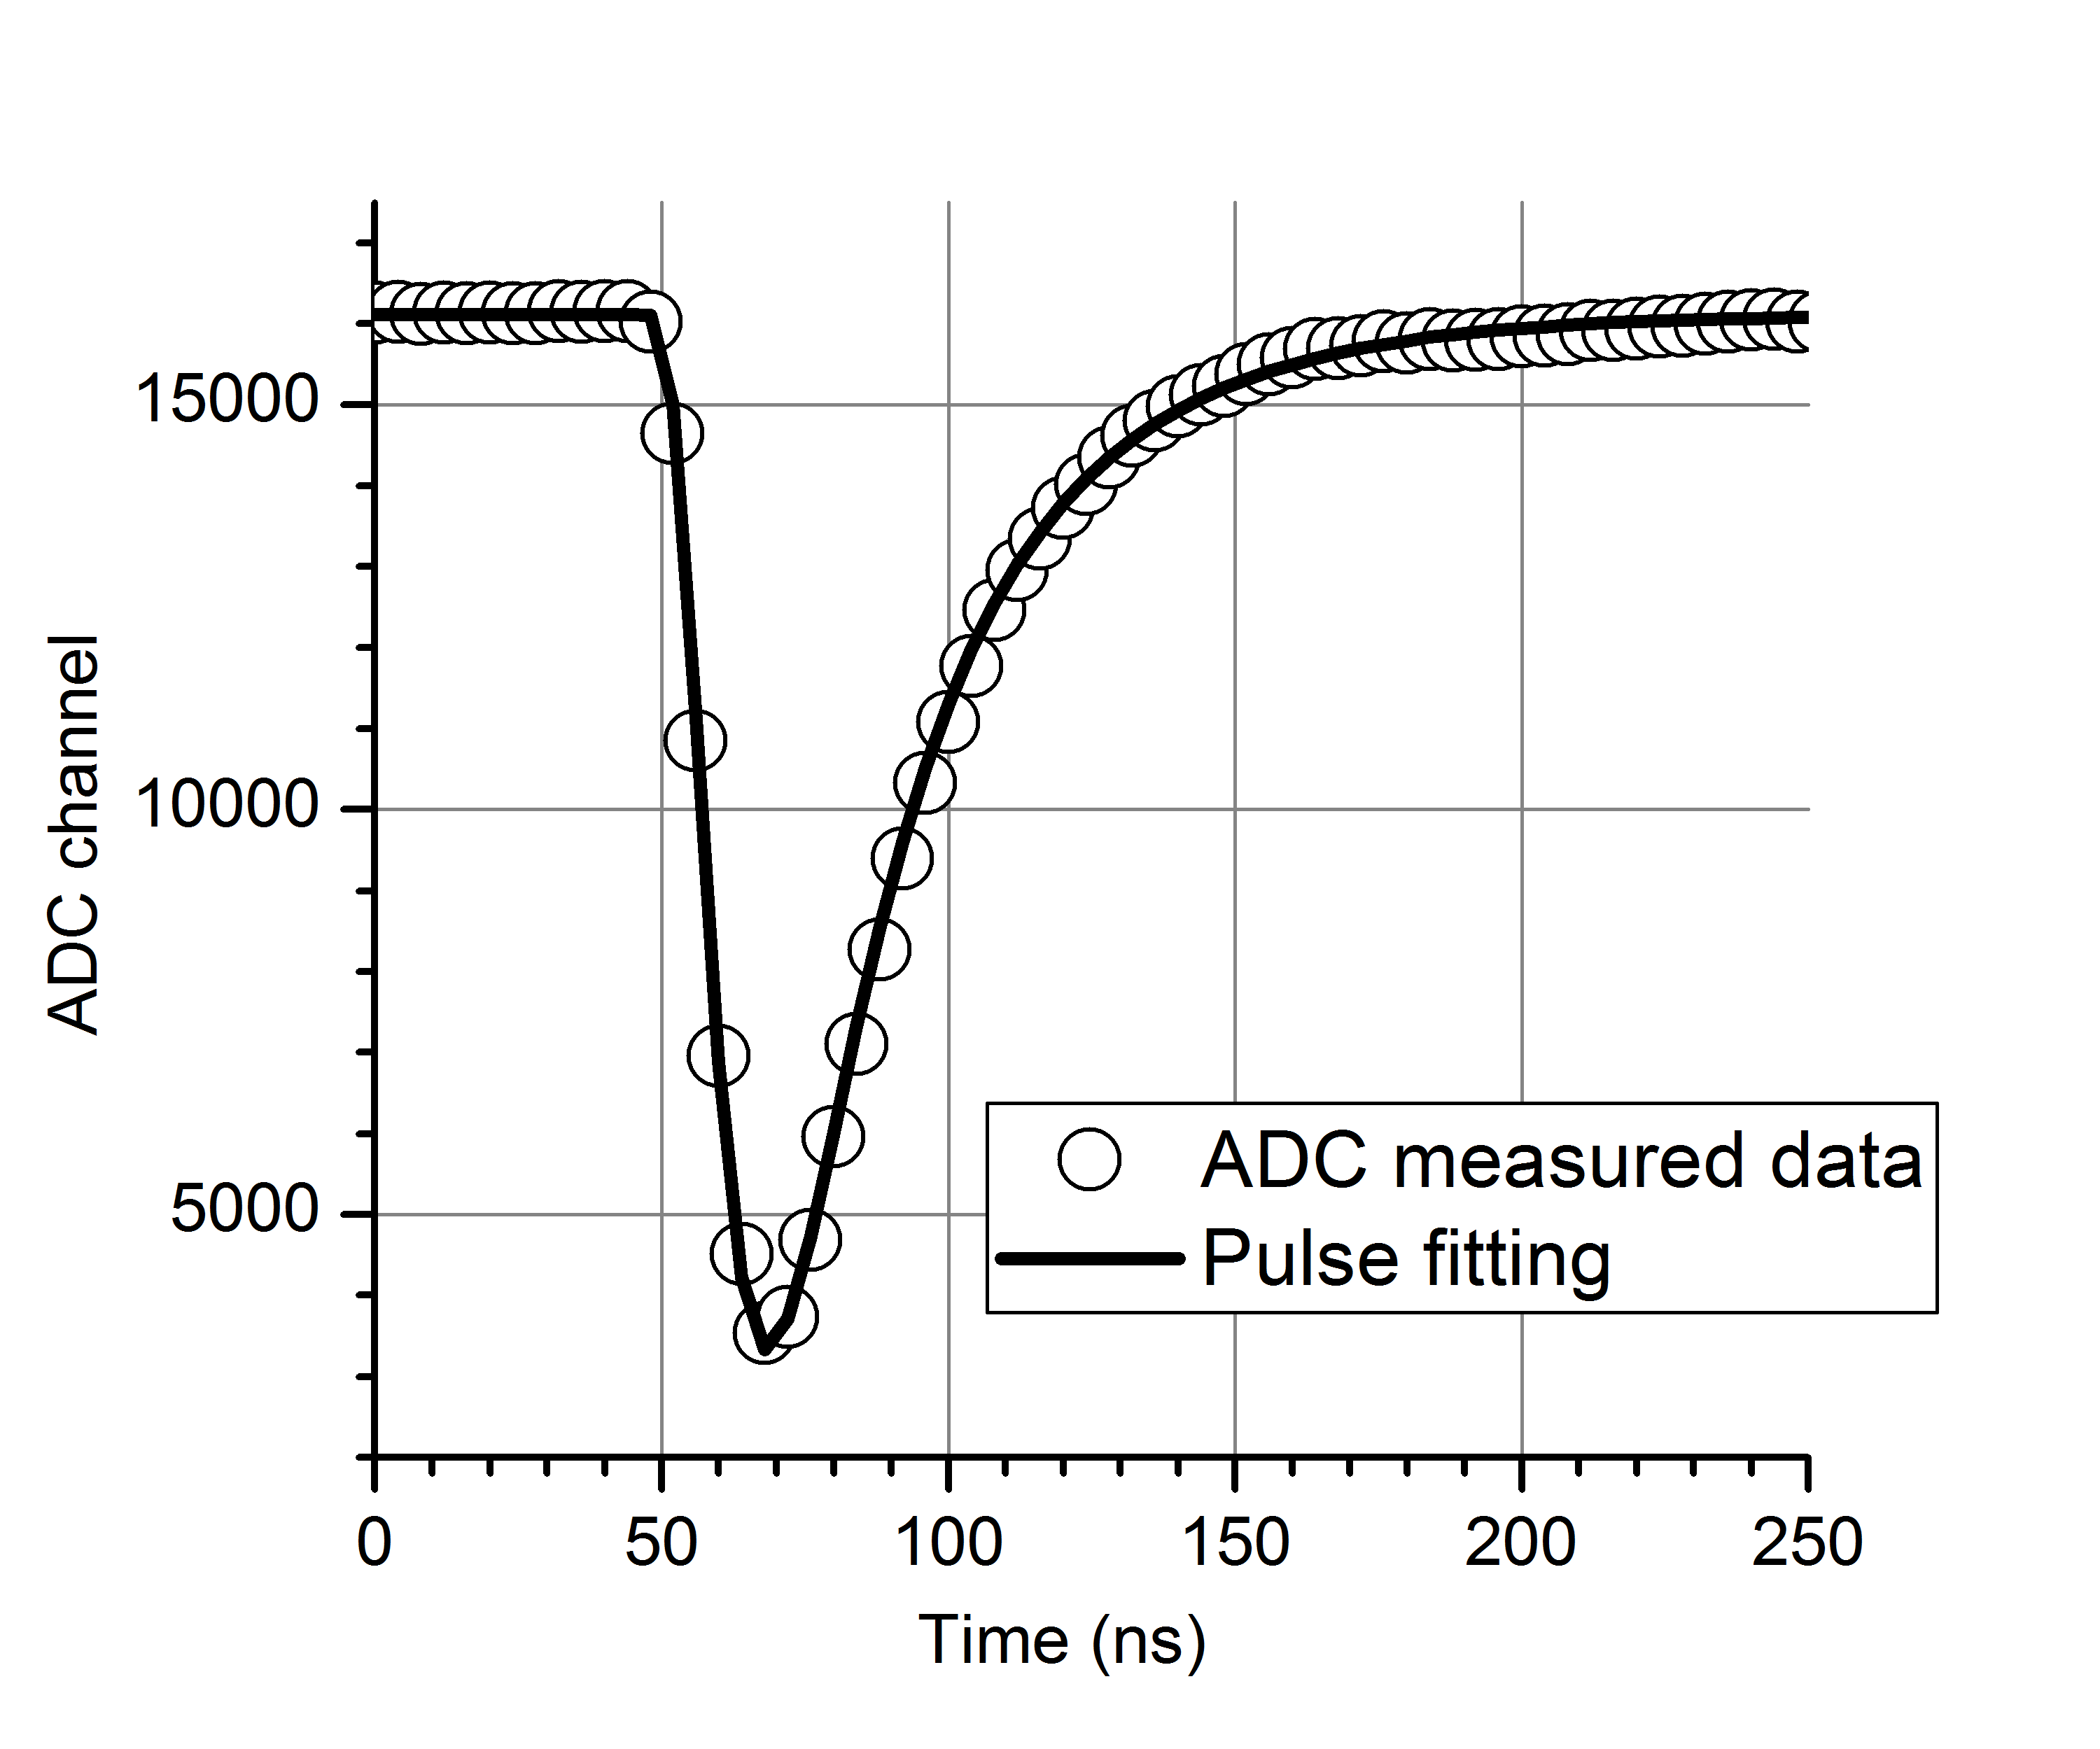
\includegraphics[width=0.60\linewidth]{pulseShapeFt2} }
  \caption{ Единчиный импульс, зарегистрированный детектором LaBr3(Ce) во время измерений на токамаке ФТ-2, а так же его аппроксимация аналитической формулой~\cite{Khilkevitch2020}.}
  \label{fig:pulseShapeFt2}
\end{figure}

\begin{figure}[ht!]
  \centerfloat{ 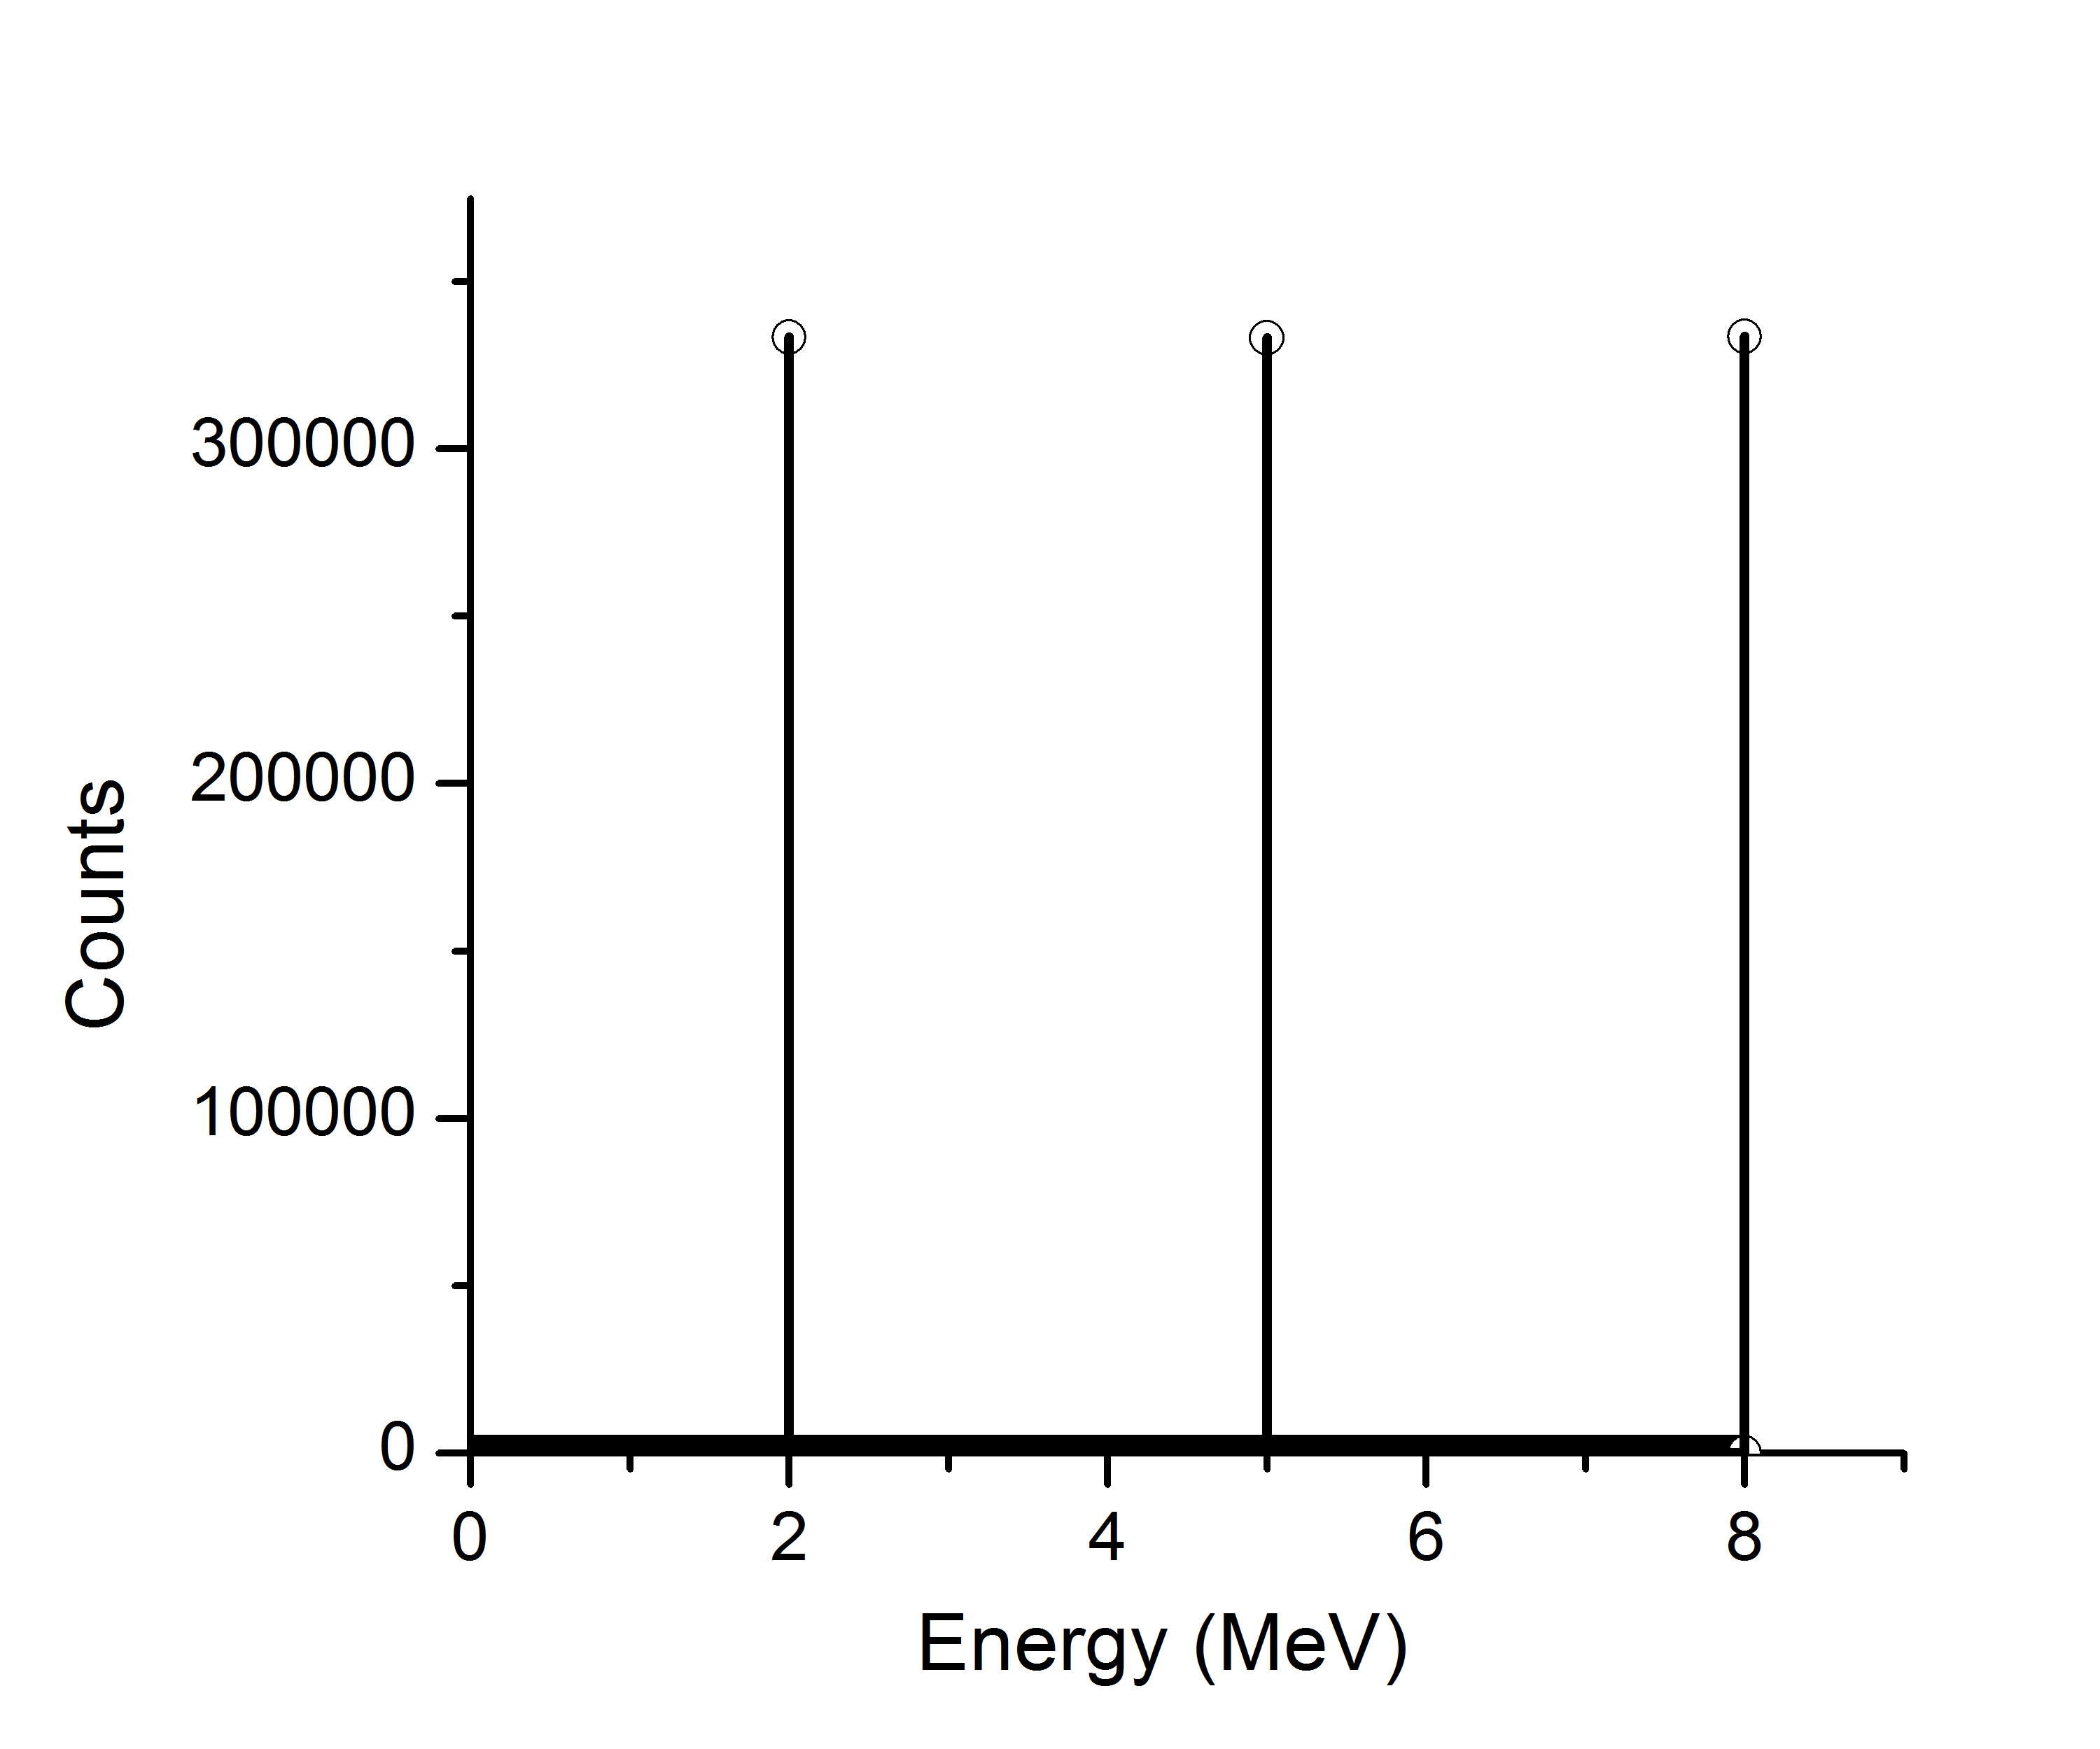
\includegraphics[width=0.60\linewidth]{testModelSpectrum} }
  \caption{ Распределение событий по энергии, которое использовалось при создании модельных сигналов~\cite{Khilkevitch2020}.}
  \label{fig:testModelSpectrum}
\end{figure}

\begin{figure}[ht!]
  \centerfloat{ 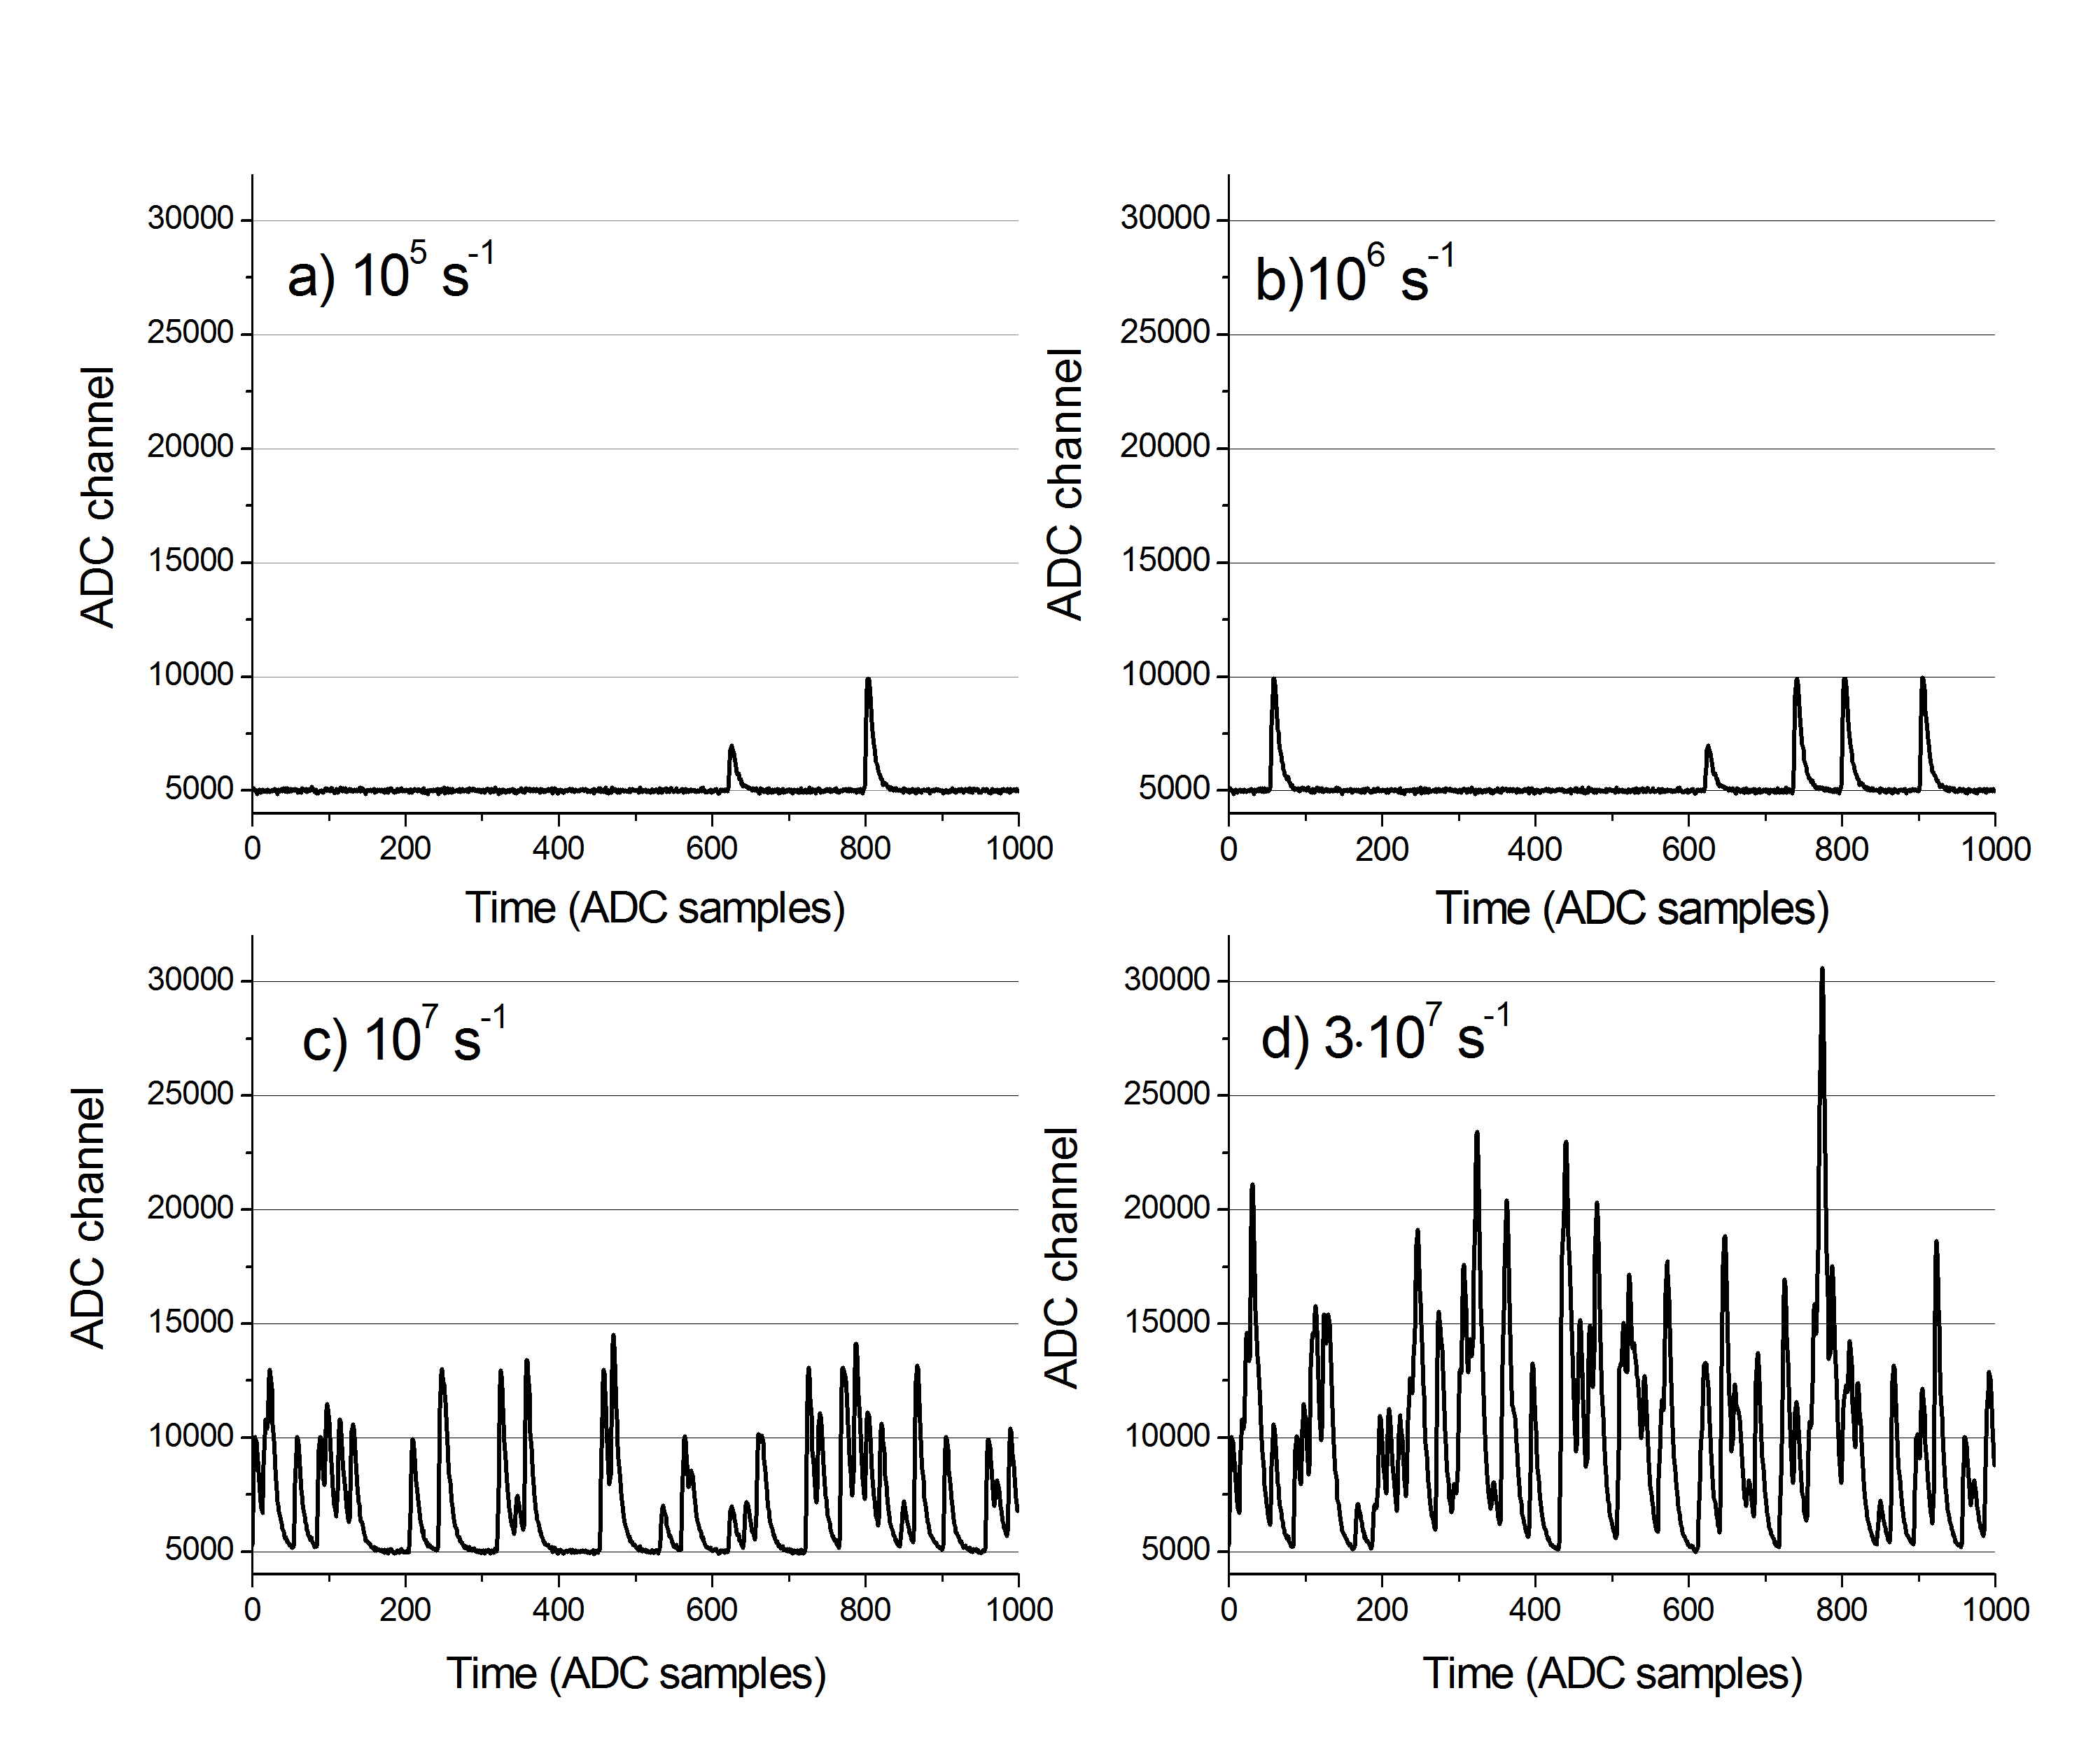
\includegraphics[width=0.96\linewidth]{testModelSignal} }
  \caption{ Модельные сигналы с разной скоростью счета: $10^5$~с${}^{-1}$~(a), $10^6$~с${}^{-1}$~(b), $10^7$~с${}^{-1}$~(c), $3\times10^7$~с${}^{-1}$~(d). При генерации использовалось одинаковое начальное значение генератора случайных чисел, поэтому по мере увеличения нагрузки в осциллограмму добавлялись новые события, а существующие события сохранялись.~\cite{Khilkevitch2020}.}
  \label{fig:testModelSignal}
\end{figure}

Для тестирования был сгенерирован набор модельных сигналов со скоростями счета $10^5$, $10^6$, $3\times10^6$, $10^7$, $2\times10^7$ и $3\times10^7$ импульсов в секунду (с${}^{-1}$). Моделирование проводилось для сигналов длительностью $t_{max} = 0.1$~с, генерируемых с частотой дискретизации 250~МГц. Использовался шум с гауссовым распределением $\sigma_n = 50$ и постоянным базовым значением $z = 5000$. События были случайным образом распределены во времени. Тестовые сигналы были откалиброваны для 1000~отчётов АЦП, соответствующих энергии гамма-излучения 1~МэВ --- по порядку величины это близко к реально используемым параметрам детектора (так, для детектора на токамаке ФТ-2 калибровка составляет примерно 1800 отсчётов на 1~МэВ). При калибровке полный диапазон энергий, измеряемый 14-разрядным АЦП, равнялся 16~МэВ. Это значение примерно соответствовало типичным параметрам, выбранным для измерения на токамаках ФТ-2 \cite{Shevelev2016,Shevelev2017} и Туман-3М \cite{Shevelev2018}. Сигналы генерировались с дискретным распределением амплитуды, показанным на рисунке~\ref{fig:testModelSpectrum}. Модельные сигналы для различных нагрузок показаны на рисунке~\ref{fig:testModelSignal}.  \cite{Khilkevitch2020}

% ==========================================================

\section{Определение нулевого уровня}

Определение нулевого уровня сигнала необходимо для дальнейшего применения методов обработки сигнала. Метод определения базовой линии должен работать при высоких скоростях счета, когда значение сигнала обычно $s(t) \gg z + n(t)$. Если значение нулевой линии во время измерения изменяется незначительно, можно использовать заданное вручную постоянное значение нулевой линии или, при обработке сигнала разряда токамака, нулевую линию можно определить автоматически в начале сигнала при низкой нагрузке детектора. Однако на практике значение нулевой линии в некоторых ситуациях существенно меняется во время разряда, например, из-за медленных периодических наводок от различного оборудования токамаков. В этом случае необходимо проводить периодические коррекции значения нулевой линии, и определять его динамически.

Целесообразно не искать значение нулевой линии в каждой точке сигнала, а ограничится периодическим определением этого значения через каждые $N_{zp}$ отсчетов АЦП. Это сокращает время обработки и позволяет отслеживать медленные изменения нулевой линии с характерным временем изменения $t_z \gg N_{zp}$. Для определения нулевого уровня можно использовать отдельные интервалы, выборки сигнала размером $N_{zd} \le N_{zp}$ в начале каждого интервала из $N_{zp}$ точек. В интервале $( k \cdot N_{zp} + N_{zd} ) \ldots ((k + 1) \cdot N_{zp})$, где $k$ --- номер интервала из точек $N_{zp}$, можно считать значение нулевой линии таким же, как и в ближайшем к нему интервале, на котором происходило вычисление значения нулевой линии. \cite{Khilkevitch2020}

% ----------------------------------------------------------

\subsection{Среднее значение и медиана}

Самый простой способ определения нулевой линии --- вычислить среднее значение:
\begin{equation*}
  z_{avg} = \frac{1}{N_{zd}} \sum\limits_{i = k \cdot N_{zp}}^{  k \cdot N_{zp} + N_{zd} } s_i 
\end{equation*}
Однако при высоких загрзуках полученное таким образом значение оказывается сильно смещено при высокой загрузке детектора (это верно для униполярного сигнала; если на АЦП приходит биполярный сигнал и $ \int_{-\infty}^{+\infty} p(t) dt = 0 $, то среднее значение вполне адекватно описывает значение нулевой линии).  

Второй очевидный способ вычисления значения нулевой линии --- это медиана, то есть такое число $z_{med}$, что половина значений сигнала $s_i$ в интервале $(k \cdot N_{zp}) \ldots (k \cdot N_{zp} + N_{zd})$ больше него, а вторая половина --- меньше. Такой сопосб вычисления нулевого уровня меньше подвержен эффекту смещения, однако всё равно даёт неудовлетворительные результаты при скорости счёта $10^7$~с${}^{-1}$ и выше. \cite{Khilkevitch2020}

% ----------------------------------------------------------

\subsection{Среднее значение по выборке}

Хороший результат дает объединение среднего и медианы в следующем итерационном алгоритме, который можно назвать <<среднее по выборке>> (<<аveraging over the selection set>>). Для неупорядоченного множества значений отсчетов $P_e$, изначально включающего в себя все значения отсчетов $s_i$ в интервале $(k \cdot N_{zp}) \ldots (k \cdot N_{zp} + N_{zd})$ определяются среднее арифметическое значение $z_{avg}$ и медиана $z_{med}$. Если 
\begin{equation}
  \label{eq:AvgOverSetCondition}
  | z_{avg} - z_{med} | < \delta z
\end{equation}
где $\delta z$ --- минимальная разность (значение этой величины является параметром алгоритма), то среднее арифметическое $z_{avg}$ можно считать равным значению нулевой линией. Типичное значение $\delta z$ составляет $0.1$--$1$; меньшие значения увеличивают время работы, при этом точность определения базовой линии с помощью алгоритма является избыточной, а большие значения приводят к недостаточной точности определения базовой линии. 

Если же условие~\ref{eq:AvgOverSetCondition} оказывается не выполненным, то из набора $P_e$ удаляются <<лишние>> значения. Количество удаляемых значений составляет $\max( \rho |P_e|, 1 )$, где $|P_e|$ --- число значений в множестве $P_e$, а величина $0 < \rho < 1$ является параметром алгоритма, обычно $\rho = 0.2$. Если $z_{avg} > z_{med}$ то из набора $P_e$ удаляются самые большие значения, а если  $z_{avg} < z_{med}$ --- то самые маленькие. После чего опять происходит вычисление $z_{avg}$ и $z_{med}$ для уменьшенного набора, и проверяется критерий~\ref{eq:AvgOverSetCondition}. Процедура повторяется до тех пор, пока этот критерий не будет выполнен. Алгоритм завершается за конечное число итераций, потому что на каждом шаге число значений в множестве $P_e$ уменьшается, а при $|P_e| = 1$ условие~\ref{eq:AvgOverSetCondition} оказывается выполнено автоматически. \cite{Khilkevitch2020}

Заметим, что для сигнала без событий $z_{avg} \approx z_{med}$. Регистрируемые события приводят к тому, что значения $z_{avg}$ и $z_{med}$ начинают смещаться от значения нулевой линии (для положительных импульсов --- в большую сторону, для отрицательных --- в меньшую). Величина смещения различается: среднее значение смещается больше, чем медиана. В данном алгоритме на каждом шаге из набора значений $P_e$ удаляются значения, вызывающие наибольшее смещение, то есть вершины импульсов. После удаления таких значений величины $z_{avg}$ и $z_{med}$ оказываются ближе к истинному значению нулевой линии. 

Работа алгоритма для участка модельного сигнала показана на рисунке~\ref{fig:baselineMethodAvgOverSet}. На первой итерации вычисления происходят для всех точек, $z_{avg} = 6921$, $z_{med} = 5969$. На второй итерации отбрасывается 20\% точек сигнала с самыми большими значениями, $z_{avg} = 5972$, $z_{med} = 5489$ --- значения стали ближе друг к другу и ближе к истинному значению нулевой линии. На третьей итерации отбрасывается ещё 20\% точек сигнала с самыми большими значениями, $z_{avg} = 5258$, $z_{med} = 5141$. На восьмой итерации $z_{avg} = 5013.02$, $z_{med} = 5013.0$, то есть значения $z_{avg}$, $z_{med}$ почти совпали; для $\delta z = 0.2$ алгоритм сходится за 8~итераций для данного участка сигнала.~\cite{Khilkevitch2020}

\begin{figure}[ht!]
  \centerfloat{ 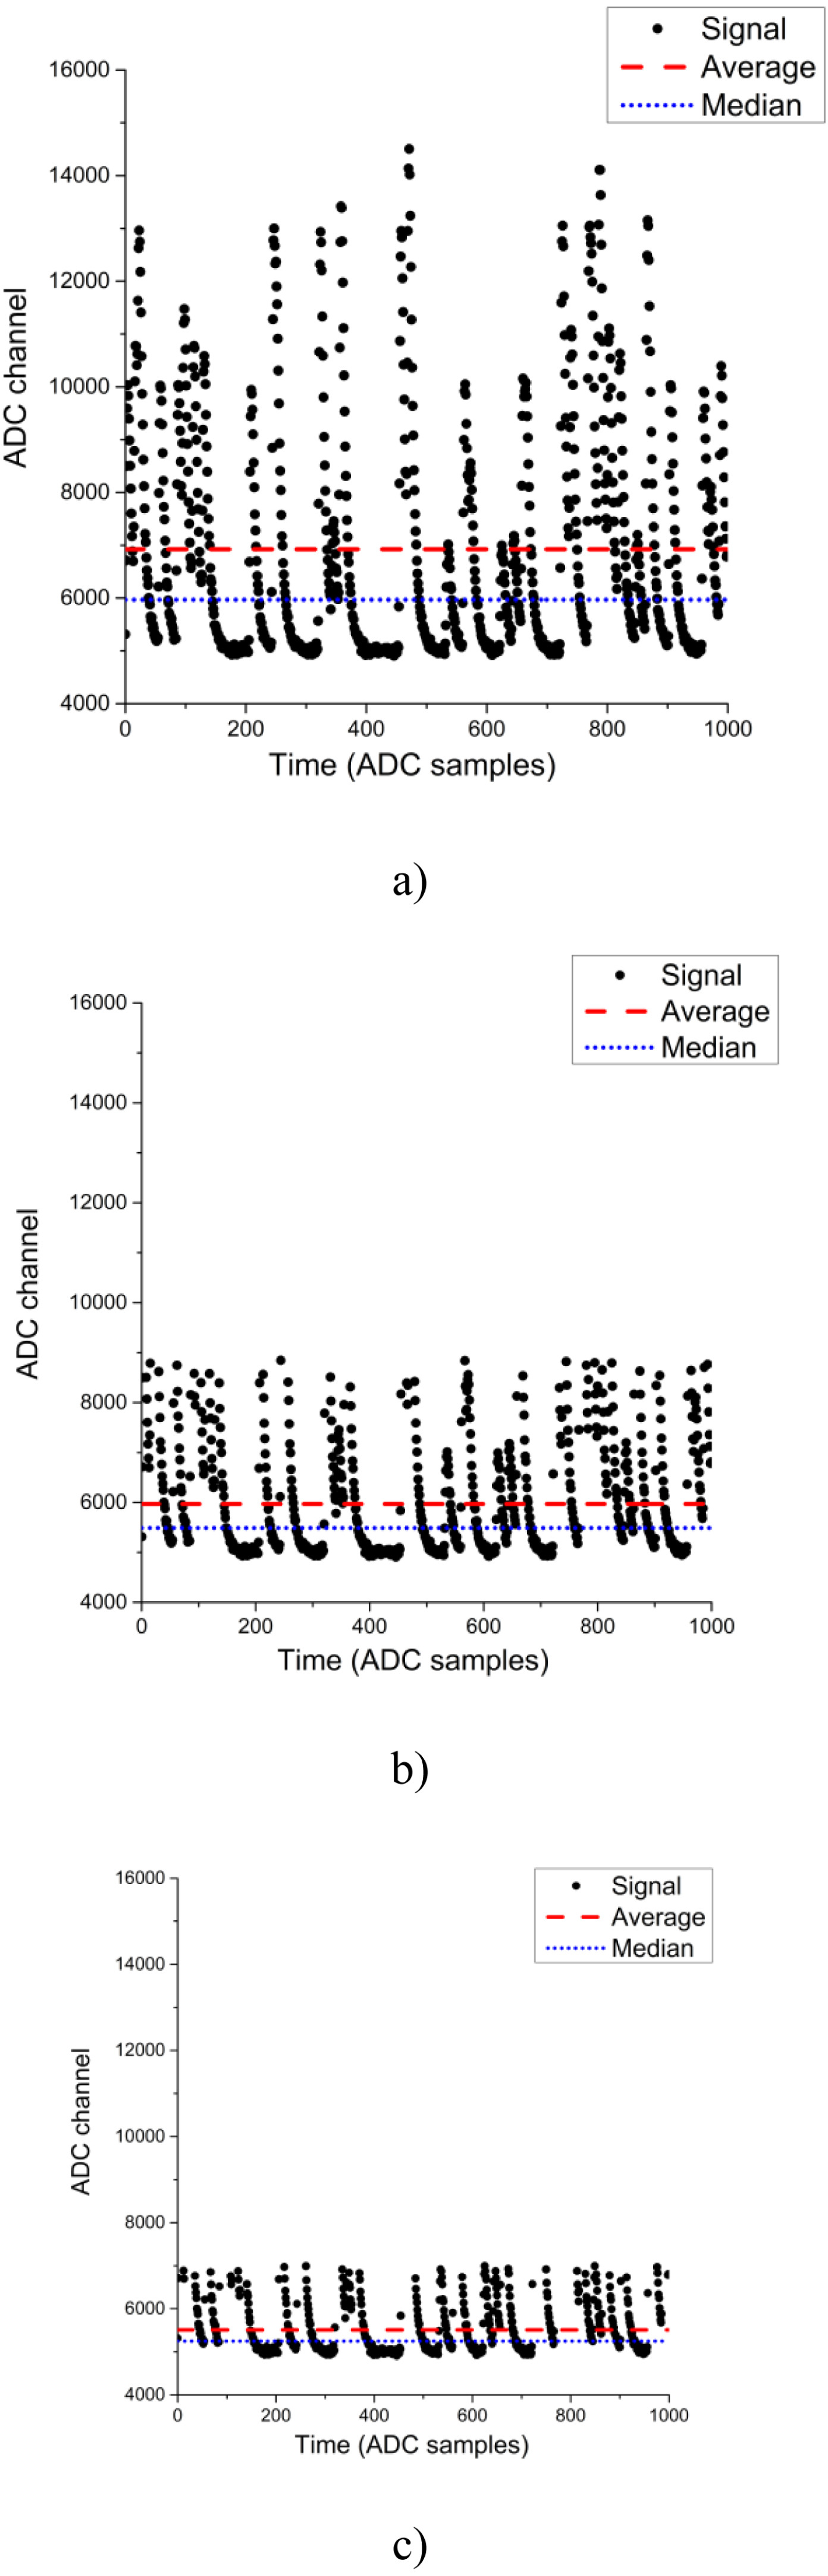
\includegraphics[width=0.40\linewidth]{baselineMethodAvgOverSet} }
  \caption{ Работа алгоритма <<среднее по выборке>> на примере участка модельного сигнала длиной 1000~точек с загрузкой $10^7$~с${}^{-1}$. Значение нулевой линии равно 5000. Чёрными точками обозначен сигнал, красным пунктиром --- среднее значение, синий линией --- медианное значение. Показаны первые три итерации алгоритма (рисуики а--в).~\cite{Khilkevitch2020}}
  \label{fig:baselineMethodAvgOverSet}
\end{figure}

% ----------------------------------------------------------

\subsection{Среднее значение по выборке плоских участков сигнала}

Описанный выше алгоритм <<среднего по выборке>> можно усовершенствовать, если из сигнала предварительно выделить плоские фрагменты (т.е. области, на которые не попадает значимый уровень сигнала от импульсов). Для этого в исходный набор данных $P_e$ для алгоритма включаются только те отсчеты $i$, для которых выполнены условия
\begin{equation}
  \label{eq:baselineMethodAvgOverFlatSet}
  \left|  s_i - \frac{1}{N_w} \sum \limits_{j=i-N_w}^{i-1} s_j  \right| < r, \hspace{5mm}
  \left|  s_i - \frac{1}{N_w} \sum \limits_{j=i+1}^{i+N_w} s_j  \right| < r 
\end{equation}
где $r$ --- пороговое значение (параметр алгоритма, выбранное типичное значение, которое больше уровня шума, но меньше чем характерный интервал между точками на фронте импульса), $N_w$ --- размер плоского участка импульса (параметр алгоритма, типичное значение 3--10), $N_w \ll N_{zd}$. Таким образом, в выборку попадают только значения таких точек, где значение сигнала лишь немного (на величину $r$) отличается от среднего уровня впереди и позади него, то есть только отсчеты, расположенные на достаточно ровных участках сигнала длительностью не более $2 \cdot N_w$. Затем к множеству таких значений применяется описанный выше алгоритм <<среднего по выборке>>. Этот метод можно назвать <<средним по выборке плоских участков>> (<<averaging over the flat chunk selection set>>). Иллюстрация работы алгоритма представлена на рисунке~\ref{fig:baselineMethodAvgOverFlatSet}.~\cite{Khilkevitch2020}

\begin{figure}[ht!!]
  \centerfloat{ 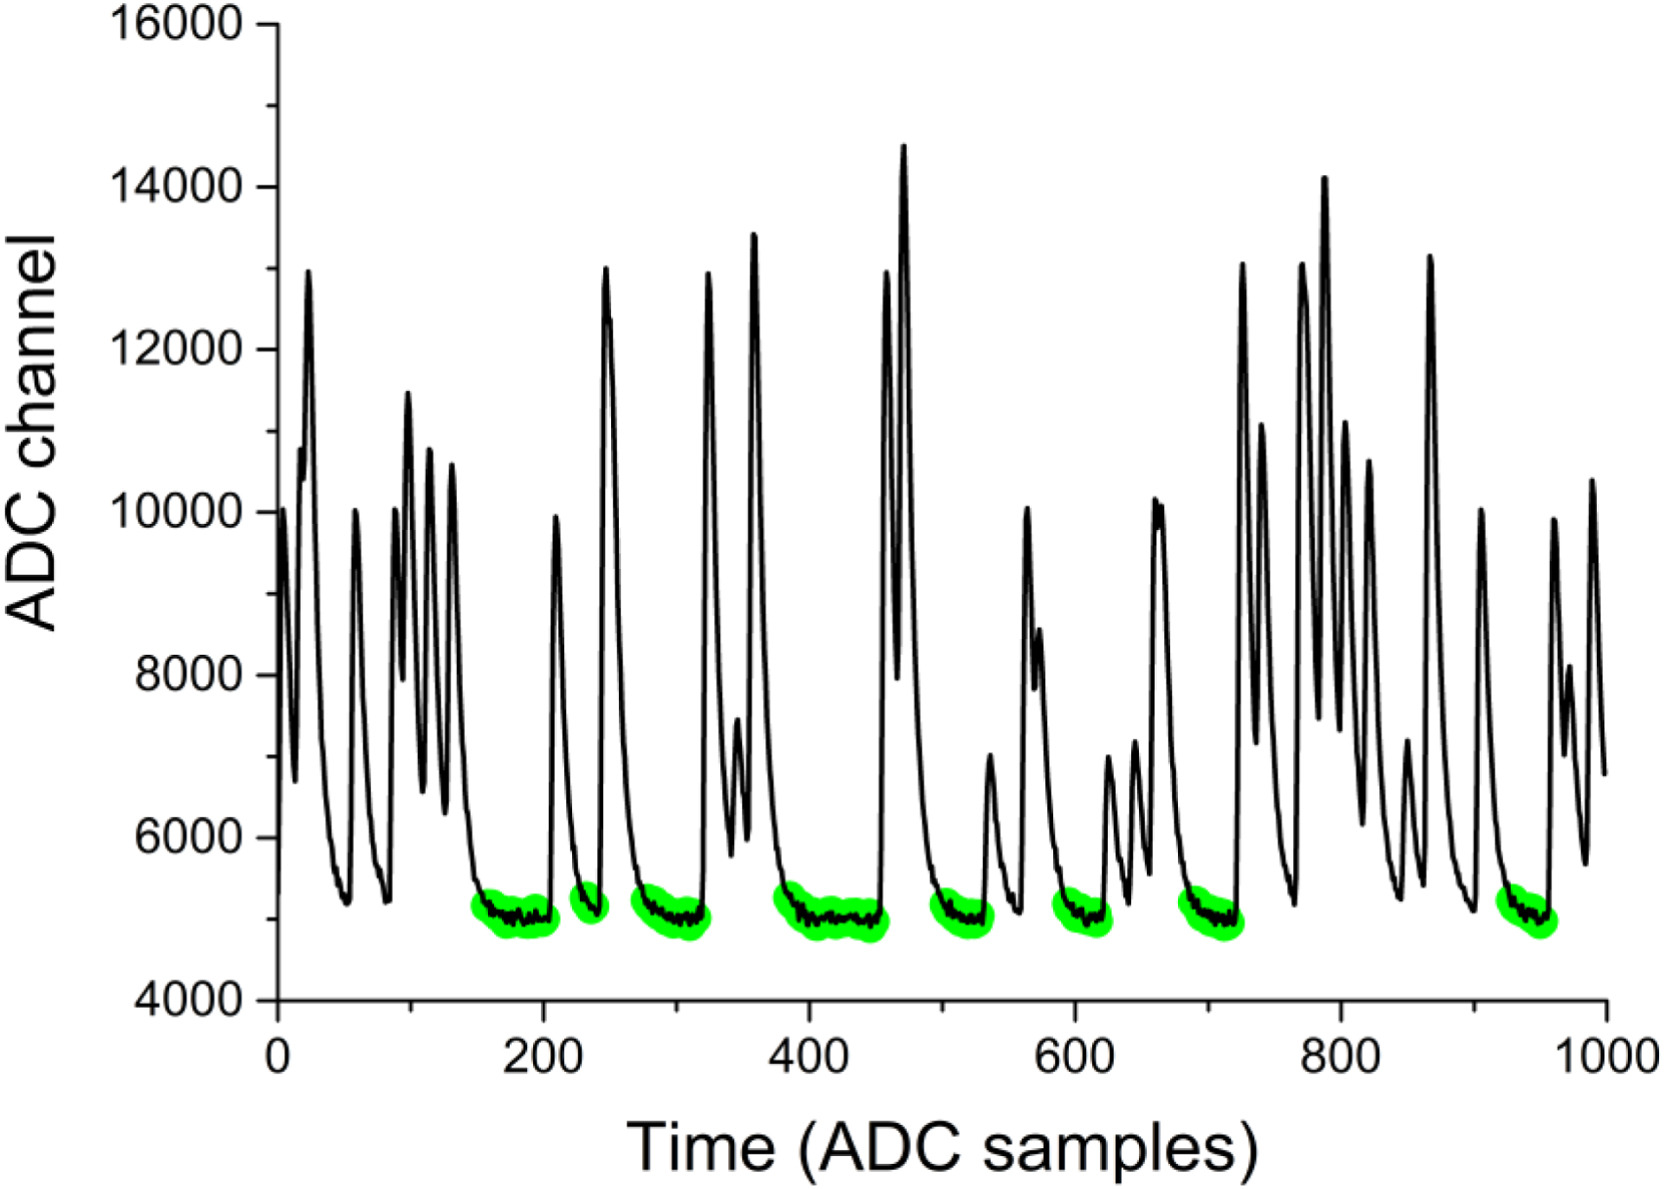
\includegraphics[width=0.50\linewidth]{baselineMethodAvgOverFlatSet} }
  \caption{ Работа алгоритма <<среднее по выборке плоских участков>> на примере участка модельного сигнала длиной 1000~точек с загрузкой $10^7$~с${}^{-1}$. Значение нулевой линии равно 5000. Чёрными точками обозначен сигнал, зелёным подсвечены участки сигнала, точки в которых удовлетворяют критерию~\ref{eq:baselineMethodAvgOverFlatSet}.~\cite{Khilkevitch2020}}
  \label{fig:baselineMethodAvgOverFlatSet}
\end{figure}

% ----------------------------------------------------------

\subsection{Сравнение методов определения значения нулевой линии}

Сравнение описанных выше методов показано на рисунке~\ref{fig:baselineMethodsComparison} при разных значениях скорости счета. Ошибка определения базовой линии равна абсолютной величине разницы между известным сгенерированным значением базовой линии модельного сигнала ($z = 5000$) и значением, полученным с помощью описанных выше алгоритмов. Наилучшие результаты демонстрирует алгоритм <<среднее по выборке плоских участков>>. При загрузке детектора $3 \times 10^7$ с${}^{-1}$ и выше погрешности определения базовой линии оказываются неприемлемо велики для всех алгоритмов, так как погрешность определения нулевой линии превышает 200 отсчётов при использовании любого рассмотренного алгоритма для выбранных событий. Это происходит из-за того, что при настолько значительной скорости счёта детектора в осциллограмме почти нет участков, где значение сигнала равно $s(t) \approx z + n(t)$ без влияния импульсов от регистрации гамма квантов.

\begin{figure}[ht!]
  \centerfloat{ 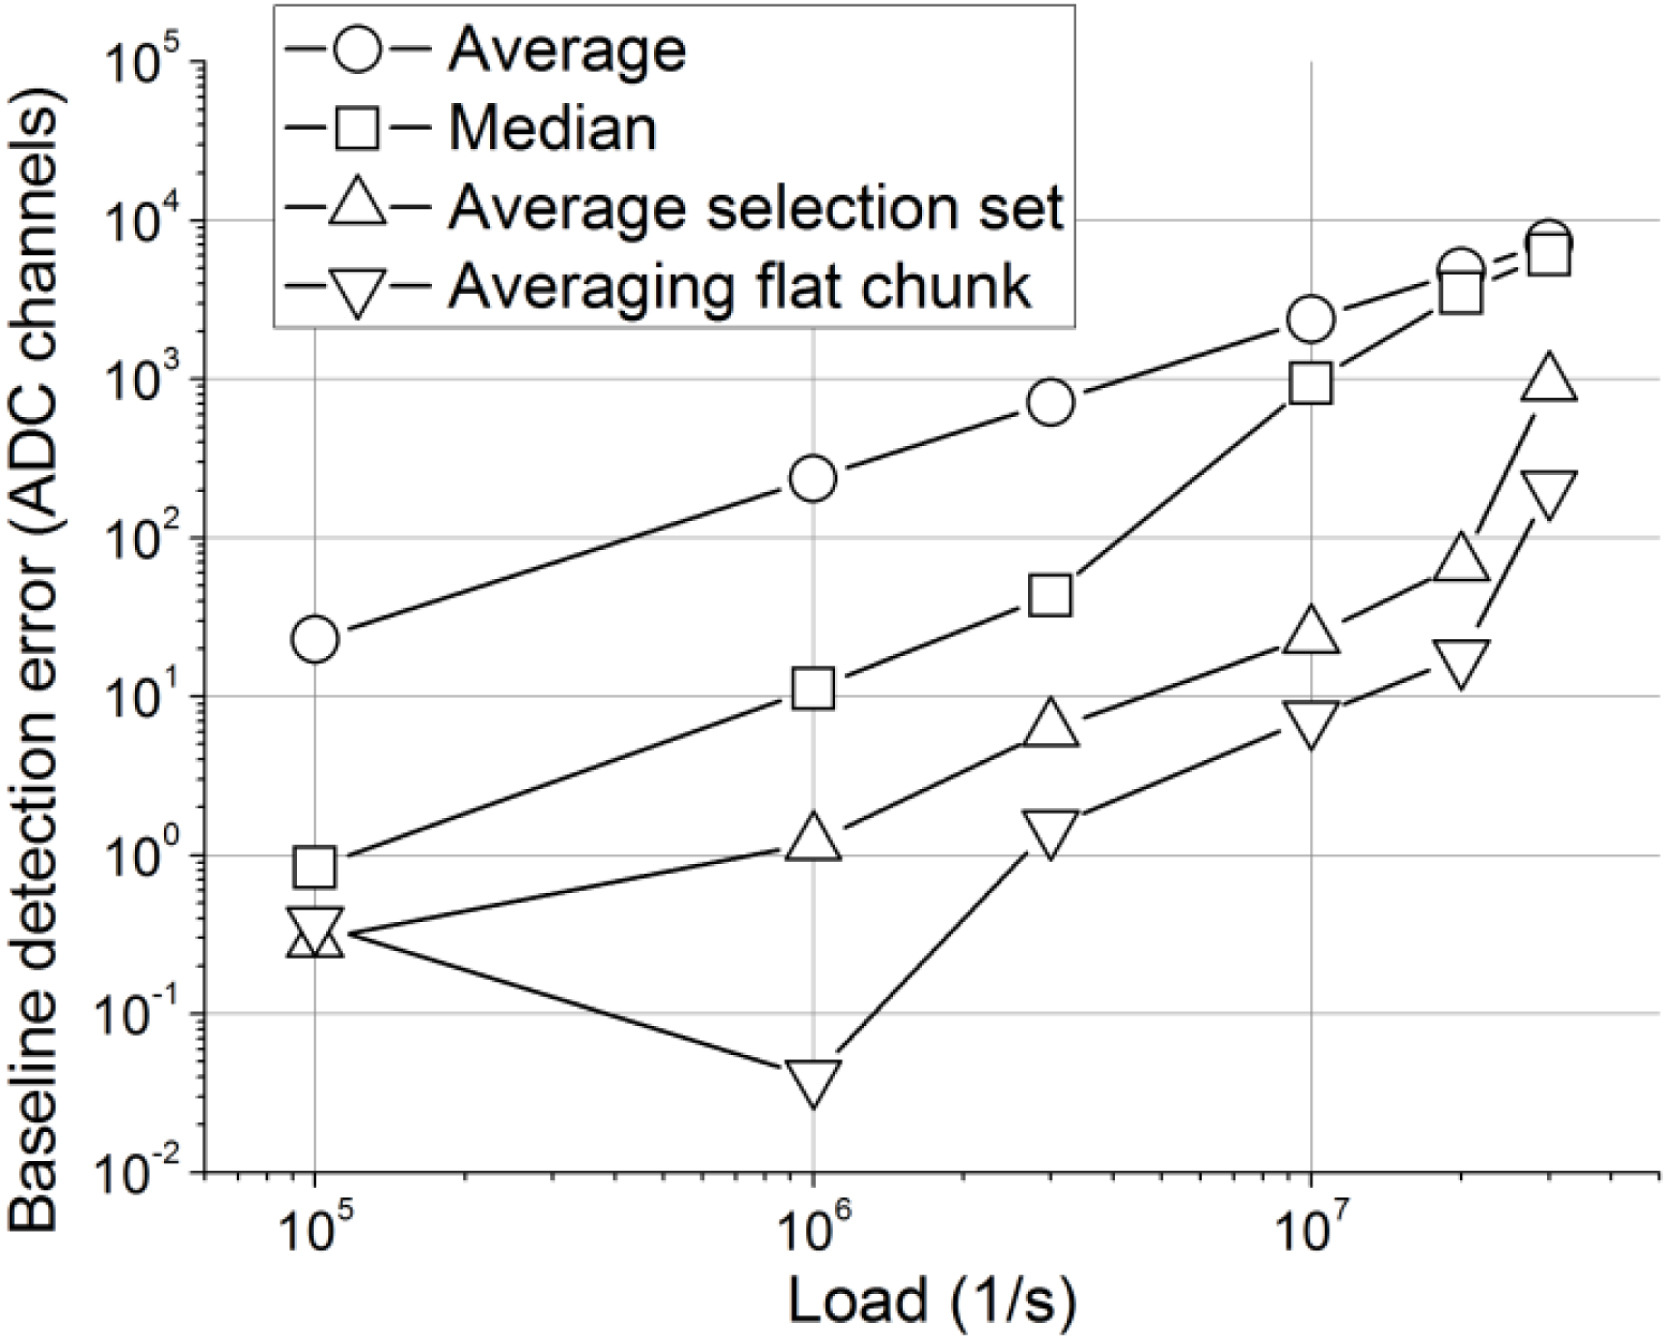
\includegraphics[width=0.60\linewidth]{baselineMethodsComparison} }
  \caption{ Ошибка в определении базового значения, полученного для различных нагрузок с использованием различных алгоритмов. По оси~Y показана ошибка в каналах АЦП модельного сигнала. Параметры алгоритмов: $N_{zd} = 10000$, $\delta z = 0.2$, $N_w = 10$, $r = 30$.  Немонотонное поведение ошибок алгоритма <<средним по выборке плоских участков>> объясняется случайными флуктуациями. В немонотонной области значение ошибки составляет менее $0.01$ отсчетов АЦП и пренебрежимо мало на практике.~\cite{Khilkevitch2020}}
  \label{fig:baselineMethodsComparison}
\end{figure}

\FloatBarrier

% ==========================================================

\section{Определение амплитуд и времени регистрации гамма квантов}

Перед определением амплитуд и времени регистрации импульсов из сигнала $s(t)$ вычитается значение нулевой линии $z$, определяемой по одному из ранее описанных алгоритмов. В дальнейшем будем считать, что определение и вычитание нулевой линии уже выполнено, поэтому $z = 0$. Предполагается, что форма импульса описывается известным уравнением и равна $p(t)$. Предполагается также, что $p(0) = 1$, $\forall t: p(t) \le p(0)$ --- импульс нормирован так, чтобы его максимальное значение было равно 1, и максимум достигался при значении $t = 0$. Для каждого события необходимо найти значения $t_j$ и $A_j$ из выражения~\ref{eq:OscShapeBase}.~\cite{Khilkevitch2020}

% ----------------------------------------------------------

\subsection{Максимальное значение}

Самый простой способ определить амплитуды событий --- найти максимальное значение импульса. Для сигнала $s_i$ необходимо найти все интервалы индексов $B_j \ldots E_j$, для которых которых $\forall i \in \left[ B_j \ldots E_j \right]: |s_j| > r$, где $r$ --- пороговое значение дискриминации. Также необходимо найти локальный максимум на каждом из этих интервалов. Это максимальное значение считается равным амплитуде события $A_j$, а время, при котором сигнал достигает локального максимума, равно времени регистрации события $t_j$.

Этот алгоритм прост и демонстрирует очень хорошую скорость обработки сигнала. Однако даже при небольшой нагрузке он обеспечивает посредственное определение истинных амплитуд импульсов, так как найденное значение чувствительно к шуму сигнала. Также из-за дискретности АЦП даже в сигнале без шумовой составляющей значение $t_j$, определённое таким образом, может отличаться на один отсчет от истинного значения времени регистрации сигнала и, соответственно, это приводит к ошибке определения амплитуды, поскольку в таком случае $ \max_{ti} p(t_i - t_j ) < 1 $. Кроме того, этот алгоритм не может адекватно определить амплитуды наложенных импульсов. Поэтому при больших загрузках определённые с помощью такого алгоритма значения $(t_j, A_j)$ будут значительно отличаться от истинных.~\cite{Khilkevitch2020}

% ----------------------------------------------------------

\subsection{Сумма}
\label{sec:ProcessingSum}

Для исключения влияния шума на результаты расчета амплитуды можно использовать и сумму отсчётов по импульсу в интервале:
\begin{equation*}
  S_j = \sum \limits_{i = B_j}^{E_j} s_i
\end{equation*}
Эта сумма зависит от того, какая часть импульса попадает в этот интервал: для импульса с большей амплитудой в интервал суммирования попадает больше точек. Поэтому имеет смысл использовать значение амплитуды импульса
\begin{equation*}
  A_j = \frac{ \sum\limits_{i=B_j}^{E_j} s_i }{ \sum\limits_{i=B_j}^{E_j} p( i - t_j ) }
\end{equation*}
где время регистрации события $t_j$ неизвестно. Приравнивание $t_j$ к времени достижения локального максимума не является точным из-за влияния возможного шума; кроме того, реальное время $t_j$ может иметь ненулевую дробную часть (т.е. событие произошло в промежутке времени между соседними сэмплами АЦП), а определённое таким образом значение заведомо является целым числом. Можно подобрать такое значение $t_j$, чтобы разность между положением центра масс измеряемого сигнала и единичной формой импульса $p(t)$ со сдвигом была минимальной:
\begin{equation*}
  \min \left( \left| \frac{ \sum \limits_{i = B_j}^{E_j} s_i \cdot (i - t_j^{max}) }{\sum \limits_{i = B_j}^{E_j} s_i} - 
                     \frac{ \sum \limits_{i = B_j}^{E_j} p( i - t_j ) \cdot (i - t_j^{max}) }{\sum \limits_{i = B_j}^{E_j} p(i - t_j) }   \right| \right) 
\end{equation*}
где $t_j^{max}$ --- время, при котором сигнал $s_i$ на интервале $\left[ B_j \ldots E_j \right] $ достигает максимального значения. 

Этот алгоритм также не может определять амплитуды наложенных импульсов. События, для которых 
\begin{equation}
  \label{eq:UnresolvedSumCrit}
  B_j - E_{j-1} < \delta i 
\end{equation}
где $\delta i$ --- параметр алгоритма (типичное значение около характерного времени спада импульса или чуть меньше), следует отбросить, так как для таких событий амплитуда второго события будет существенно искажена влиянием первого события: эти близкие события считаются неразрешёнными. Однако влияние неразрешённых событий также может быть учтено. Для таких неразрешенных событий можно оценить их суммарную амплитуду равной
\begin{equation}
  \label{eq:UnresolvedAmplitude}
  A_j^u = \frac{  \sum \limits_{i = B^u_j}^{E^u_j} s_i }{ \sum \limits_{i = -\infty}^{+\infty} p(i) }
\end{equation}
где $\left[ B_j^u \ldots E_j^u \right] $ --- объединённый интервал для всех соседних событий, не удовлетворяющих условию~\ref{eq:UnresolvedSumCrit}. Можно предположить, что распределение амплитуд неразрешенных событий примерно соответствует распределению разрешённых событий в их непосредственной близости. Для учета неразрешенных событий каждому событию присваивается вес $w_j$. При условии отсутствия неразрешённых событий этот вес изначально равен $1$ для всех событий. Однако если событие $j$ не разрешено (не соответствует критерию~\ref{eq:UnresolvedSumCrit}), то для каждого события в интервале $i_b \ldots i_e$ вблизи события $j$ этот вес увеличивается на величину
\begin{equation*}
  \Delta w = \frac{ A_j^u }{ \sum \limits_{i=i_b}^{i_e} A_i } 
\end{equation*}
Величину интервала $i_b \ldots i_e$ можно определять разными способами, например как $i_b = j - N_{uw}$, $i_e = j + N_{uw}$, где величина $N_{uw}$ --- параметр алгоритма, типичное значение, используемое нами, обычно равно 1000. При построении спектра значение в энергетическом интервале $i$ в диапазоне энергий $\varepsilon_i \ldots \varepsilon_{i+1}$ определяется как сумма
\begin{equation*}
  \sum_j w_j | \varepsilon_i \le A_j < \varepsilon_{i+1}
\end{equation*}
Аналогично при построении зависимости скорости счёта детектора от времени число событий во временном интервале $t_i \ldots t_{i+1}$ определяется как
\begin{equation*}
  \sum_j w_j | t_i \le t_j < t_{i+1}
\end{equation*}
Спектр, полученный этим методом, можно зазывать скорректированным спектром. Заметим, что построенный таким образом спектр, учитывающий неразрешённые значения, может содержать нецелые значения, в отличие от <<обычного>> спектра, где в каждом интервале содержится всегда целое число событий.~\cite{Khilkevitch2020}

% ----------------------------------------------------------

\subsection{Фиттинг по форме импульса}
\label{sec:FittingProcessing}

В качестве усовершенствованного метода определения амплитуды, обеспечивающего разделение наложенных импульсов, можно использовать подгонку (фиттинг) фрагмента осциллограммы известной формой импульса $p(t)$, в результате чего определить амплитуду и время регистрации события. Первоначальный метод был описан в \cite{Gin2008}, однако в \cite{Khilkevitch2020} он был модифицирован для повышения точности.

Будем для каждого события $j$ искать такие параметры $A_j$ и $t_j$, чтобы минимизировать невязку
\begin{equation}
  \label{eq:FittingResidual}
  R(t_j,A_j) =   \sum \limits_{i=B^f_j}^{E^f_j} \left| s'_i - A_j \cdot p( i - t_j ) \right|
\end{equation}
где $B^f_j < t_j^{max}$ и $E^f_j > t_j^{max}$ определяют интервал, в котором проводится фиттинг. Заметим, что эти значения не обязательно равны значениям $B_j$ и $E_j$. Значение 
\begin{equation*}
  s'_i = s_i - \sum \limits_{k=0}^{j-1} A_k \cdot p( i - t_k )
\end{equation*}
учитывает влияние медленно спадающих <<хвостов>> предыдущих импульсов при анализе импульса $j$. Поскольку сигнал обрабатывается последовательно, то все значения $A_k$ и $t_k$ для $k<j$ известны.

При заданном значении $t_j$ минимум невязки $R(A_j)$ может быть определён методом наименьших квадратов и равен
\begin{equation}
  \label{eq:FittingAmplitude}
  A_j = \frac{ \sum \limits_{i=B^f_j}^{E^f_j} s' \cdot p(i - t_j) }{ \sum \limits_{i=B^f_j}^{E^f_j} p^2(i-t_j) }
\end{equation}
Соответственно, необходимо найти такое значение $t_j$ на интервале $\left[ B_j \ldots E_j \right] $, такое чтобы чтобы невязка из выражения~\ref{eq:FittingResidual} со значением амплитуды их \ref{eq:FittingAmplitude} принимала наименьшее значение. Это можно сделать методом троичного поиска \cite{Scherer2017}, который, с одной стороны, работает достаточно быстро, а с другой стороны, обеспечивает достаточную для гамма-спектрометрии точность определения значения $t_j$ (обычно нам требуется знать $t_j$ с точностью не более долей единицы). Поиск ведется на дискретной сетке с шагом $1/t_v$, где целочисленное значение $t_v \ge 1$ (это параметр алгоритма, обычно используемые нами значения равны 2 или 4, оно определяется желаемой точностью определения $t_j$). Интервал поиска равен $ t_j^{max} - \Delta^b \ldots  t_j^{max} + \Delta^e$, где $\Delta^b$ и $\Delta^e$ --- параметры алгоритма, которые определяются шириной импульса и уровнем шума; обычно $\Delta^b = \Delta^e = 3..10$.

%Если для вычисленных значений  $A_j$ и $t_j$ невязка оказалась больше некоторого значения
%\begin{equation}
%  \label{eq:ResidualCondition}
%  R( A_j, t_j ) \ge R^{max}
%\end{equation}
%где  $R^{max}$ --- параметр алгоритма, обычно это значение в 2--3 раза больше уровня шума, то считается что импульс не удалось разрешить, так как его форма слишком сильно отличается от эталонной формы $p(t)$. В этом случае можно применить ту же коррекцию итогового спектра на неразрешённые импульсы, что была описана выше в разделе~\ref{sec:ProcessingSum}, и рассчитать суммарную амплитуду неразрешённых сигналов по той же формуле~\ref{eq:UnresolvedAmplitude}~\cite{Khilkevitch2020}.


Если значение невязки больше некоторого порогового значения 
\begin{equation*}
  \frac{ R(t_j,A_j) }{ E_j - B_j } > R^{max}
\end{equation*}
где $R^{max}$ --- параметр алгоритма, обычно это значение в 2--3 раза больше уровня шума, то предполагается, что форма импульса слишком сильно отличается от $p(t)$, а значения $A_j$ и $t_j$ определены неверно. Это может произойти из-за очень близкого наложения двух или более импульсов, так что хотя сигнал $s_i$ имеет только один локальный максимум в интервале $\left[ B_j \ldots E_j \right] $, но реально было зарегистрировано более одного события. В этом случае можно считать, что события не удалось разрешить. Однако и эти неразрешённые события можно учитывать так же, как и в разделе~\ref{sec:ProcessingSum}.


После определения времени и амплитуды события $j$ хвост импульса вычитается из остаточного сигнала перед его обработкой по формуле
\begin{equation*}
  s'_i = s_i - A_j \cdot p( t - t_j )
\end{equation*}
Эта процедура учитывает влияние события $j$ на последующие события.

Пример работы алгоритма показан на рисунке~\ref{fig:FittingProcessing}.

\begin{figure}[ht]
    \begin{minipage}[b][][b]{0.95\linewidth}\centering
        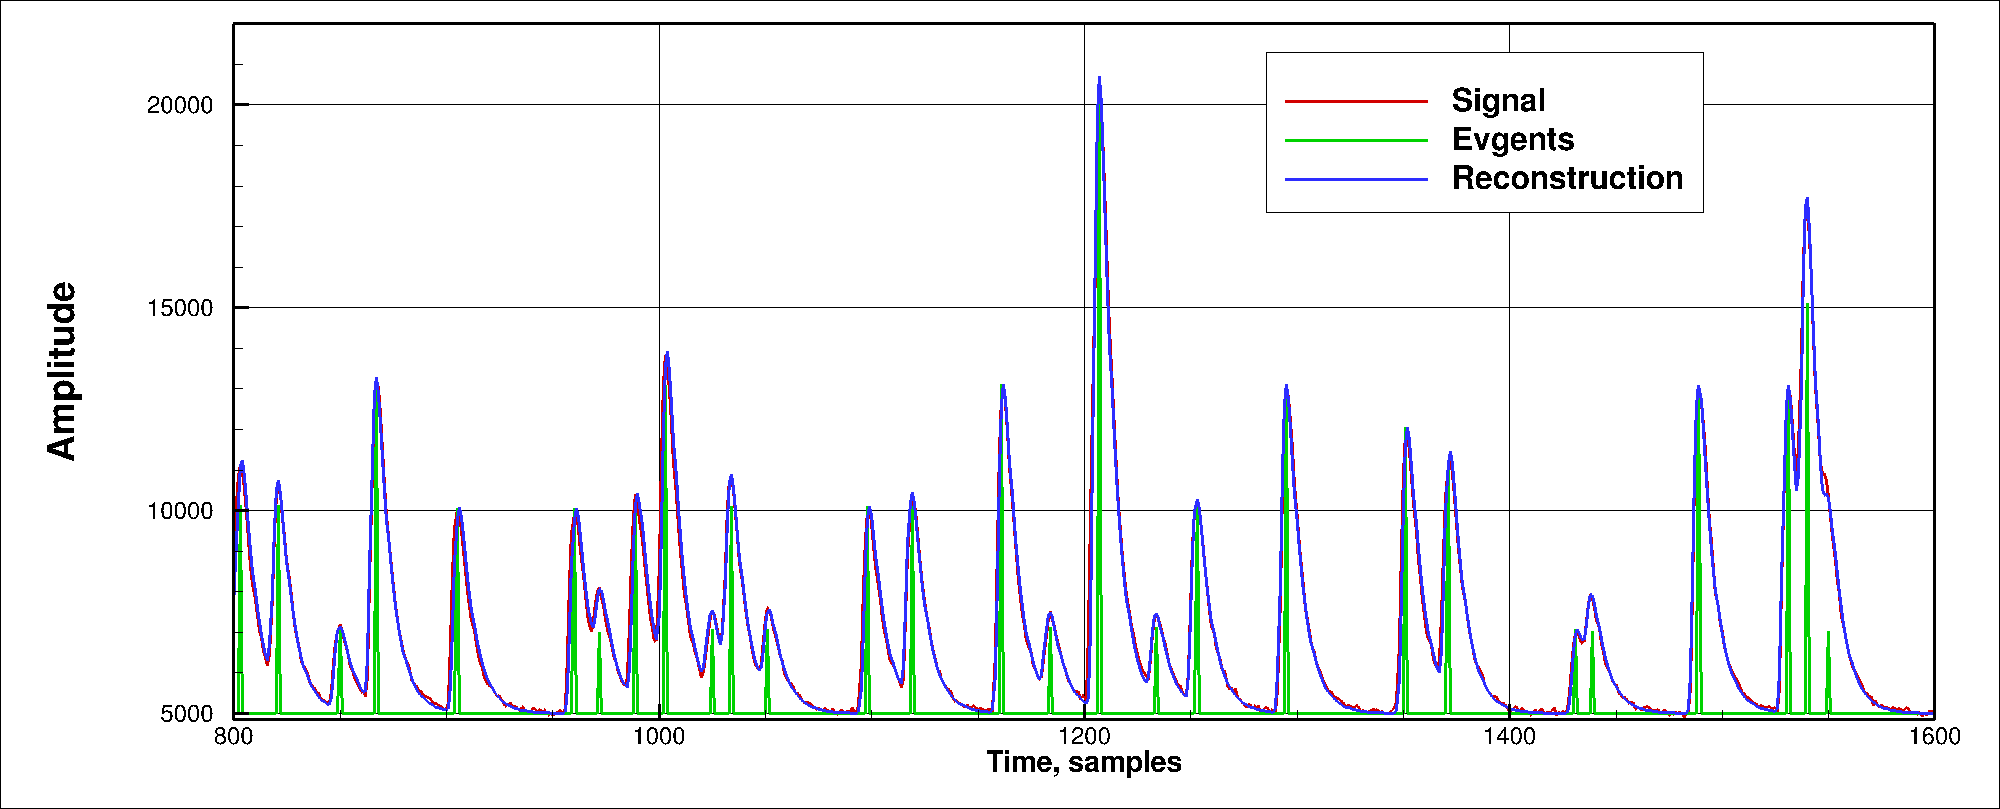
\includegraphics[width=0.95\linewidth]{fittingProcessing1e7} \\ а)
    \end{minipage}
    \vfill
    \begin{minipage}[b][][b]{0.95\linewidth}\centering
        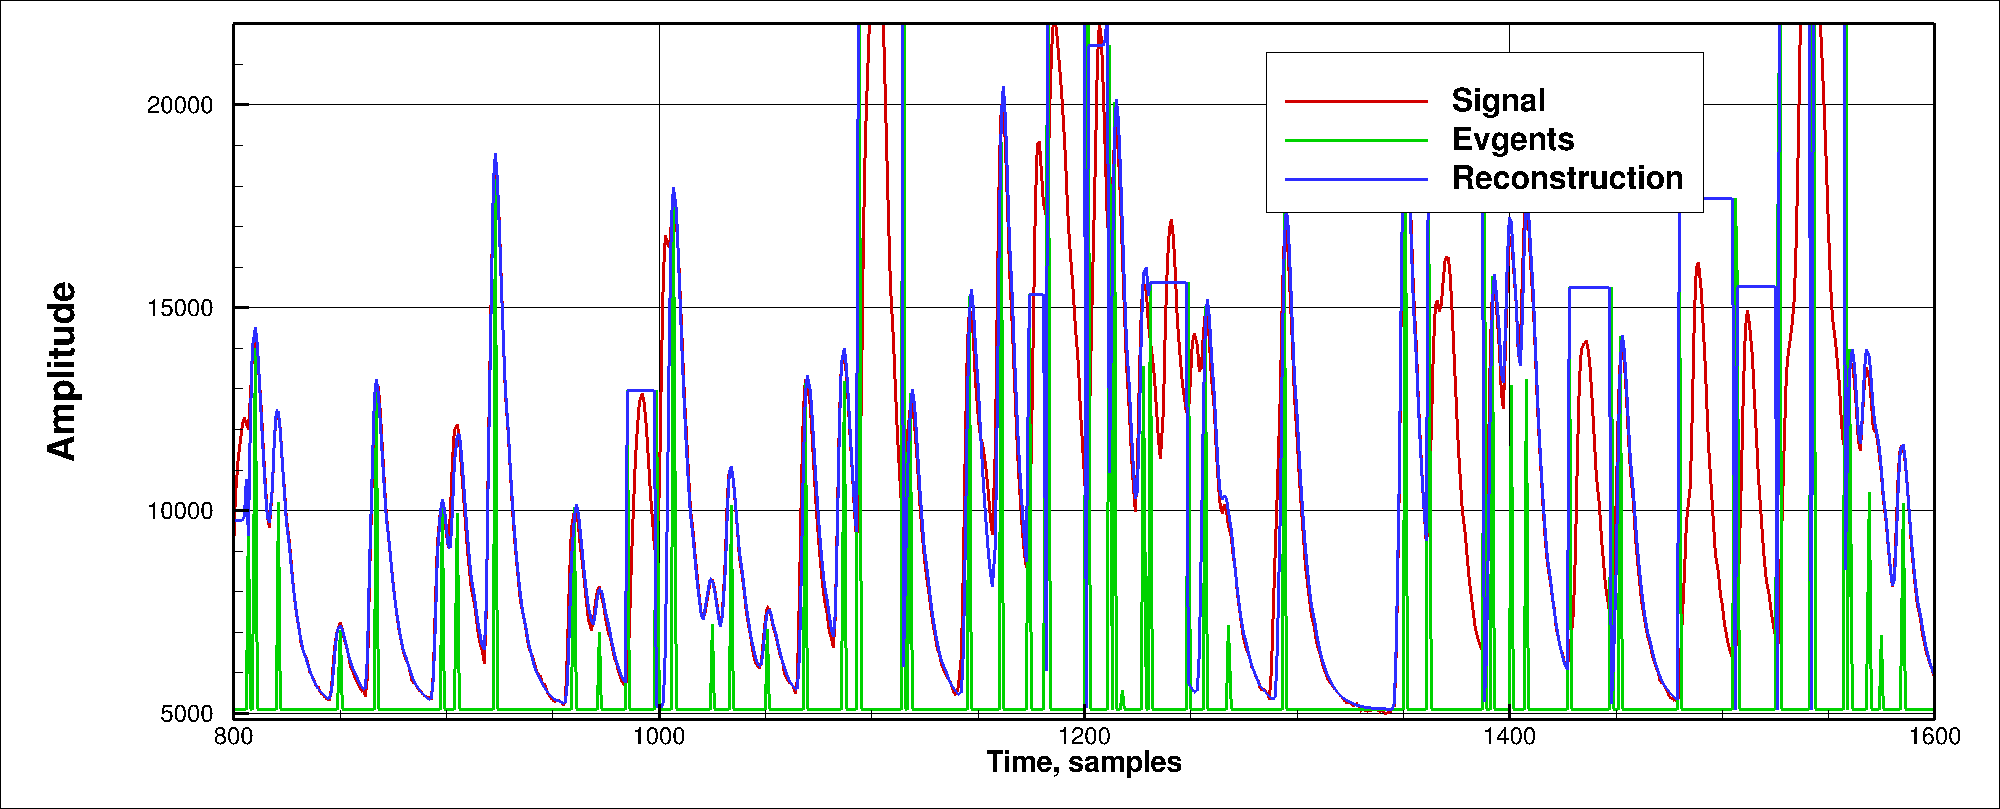
\includegraphics[width=0.95\linewidth]{fittingProcessing3e7} \\ б)
    \end{minipage}
    \vspace{5mm}
    \caption{ Пример работы алгоритма при обработке сигнала с загрузкой $10^7$~с${}^{-1}$~(а) и $3 \times 10^7$~с${}^{-1}$~(б). Красной линией обозначен модельный сигнал. Зелёным показан результат обработки сигнала с помощью алгоритма: импульсы, для которых $R/(E-B)<R^{max}$ и которые считаются успешно разобранными, представлены в виде единичных импульсов, а для импульсов, где $R/(E-B)>R^{max}$, на рисунке нарисован прямоугольник. Синим показан результат операции $z + \sum A_j p(t - t_j)$, то есть это такой сигнал, который соответствует разобранным импульсам; аналогично, для неразрешённых импульсов нарисован прямоугольник.~\cite{Khilkevitch2020}. }
    \label{fig:FittingProcessing}
\end{figure}

% ----------------------------------------------------------

\subsection{Деконволюция сигнала}

Методы деконволюции можно использовать для разделения сильно наложенных импульсов. Сигнал может быть представлен в виде свертки множества дельта-функций с ядром свертки, представляющим собой форму одиночного импульса: 
\begin{equation}
  \label{eq:SignalAsConvolution}
  s(t) = \int \limits_{-\infty}^{+\infty} p( t' - t ) \sum \limits_{i=0}{L} A_j \cdot \delta(t' - t_i) dt' + n(t)
\end{equation}
где $L$ --- количество гамма-событий. В дискретной форме, если пренебречь шумовой составляющей $n(t)$, это выражение приблизительно переписать как 
\begin{equation}
  s = P \cdot A
\end{equation}
где $s$ --- вектор отсчетов АЦП $s_i$, $P$ --- квадратная матрица свертки, $A$ --- вектор амплитуд импульсов. Значения матрицы $P$ равны
\begin{equation*}
  P_{i,j} = p( j - i )
\end{equation*}
Если время зарегистрированного события $t_j$ является целым числом, то значение вектора $A_{tj}$ равно значению амплитуды события. Если же вемя $t_j$ имеет дробную составляющую, то предполагается, что сумма двух соседних элементов вектора $A$ примерно равна амплитуде события $A_j$ при достаточно высокой частоте дискретизации АЦП по сравнению с длительностью импульса. Численный эксперимент показывает, что разница между суммой $A_{tj} + A_{tj+1}$ и истинной амплитудой $A_j$ не превышает 0.62\% для тестовой формы импульса.

Процедура деконволюции с использованием методов преобразования Фурье сложна из-за малой длительности импульса $p(t)$, часто около 20 отсчетов АЦП и менее, и желаемого дельта-образного решения~\cite{Morhac2011}. Можно использовать итерационные алгоритмы, такие как алгоритм Голда~\cite{Gold1964}. На каждой итерации этого алгоритма новое значение вычисляется как
\begin{equation*}
  A_i^k = \max \left( 0, \frac{A_i^{k-1} \cdot \widetilde{S_i} }{ \sum_{m=1}^{N} \widetilde{ P_{i,m} } \cdot A_m^{k-1} } \right)
\end{equation*}
где $k$ --- номер итерации, $\widetilde{S} = P^{T} \cdot S $, $\widetilde{P} = P^{T} \cdot P$, $N$ --- размер квадратной матрицы $P$ и вектора $A$.

В качестве начального условия можно выбирать значение сигналоа $A_i^0 = s_i$. Для обработки сигналов число итераций алгоритма можно сделать фиксированным, и равным некоторому значению, подбираемым опытным путем (например, 100~итераций). В процессе деконволюции для ускорения сходимости алгоритма через каждые несколько (например, 30) итераций можно проводить преобразование вида $A_i^k = \left( A_i^k \right)^g$, где значение степени $g$ --- параметр алгоритма, оно должно быть равным или чуть больше 1.0 (например, 1.05)~\cite{Morhac2011, Khilkevitch2020}.

На практике решение полного уравнения для всего сигнала целиком невозможно из-за чрезмерно большой размерности задачи, которая часто превышает $10^9$. Однако, поскольку функция отклика убывает, можно рассматривать за раз не весь сигнал целиком, а отдельные фрагменты сигнала, где его значение превышает порог $r$, и проводить деконволюцию только участков $\left[ B_j \ldots E_j \right] $. 

После деконволюции сигнала со значительным уровнем шума результатом является вектор $A$, в котором значения элементов часто не полностью соответствуют ожидаемым значениям: есть пики, не соответствующие никаким импульсам, которые возникли из-за шума исходного сигнала; но при этом одному реальному событию часто соответствует несколько соседних элементов вектора. Для получения амплитуд событий проводится суммирование групп соседних ненулевых значений вектора $A$. Все события меньше некоторого порога $r_A$ отбрасываются.

После вычисления амплитуд импульсов в интервале вычисляется невязка $R$. Если невязка больше определенного порогового значения $R^{max}$, то, как и в описанных выше алгортимах, можно считать что время и амплитуда событий на интервале были определены некорректно. В этом случае для коррекции спектра с учётом неразрешенных событий можно применить ту же процедуру, что и для методов фиттинга и суммирования.

Пример работы алгоритма показан на рисунке~\ref{fig:DeconvProcessing}.

\begin{figure}[ht]
    \begin{minipage}[b][][b]{0.95\linewidth}\centering
        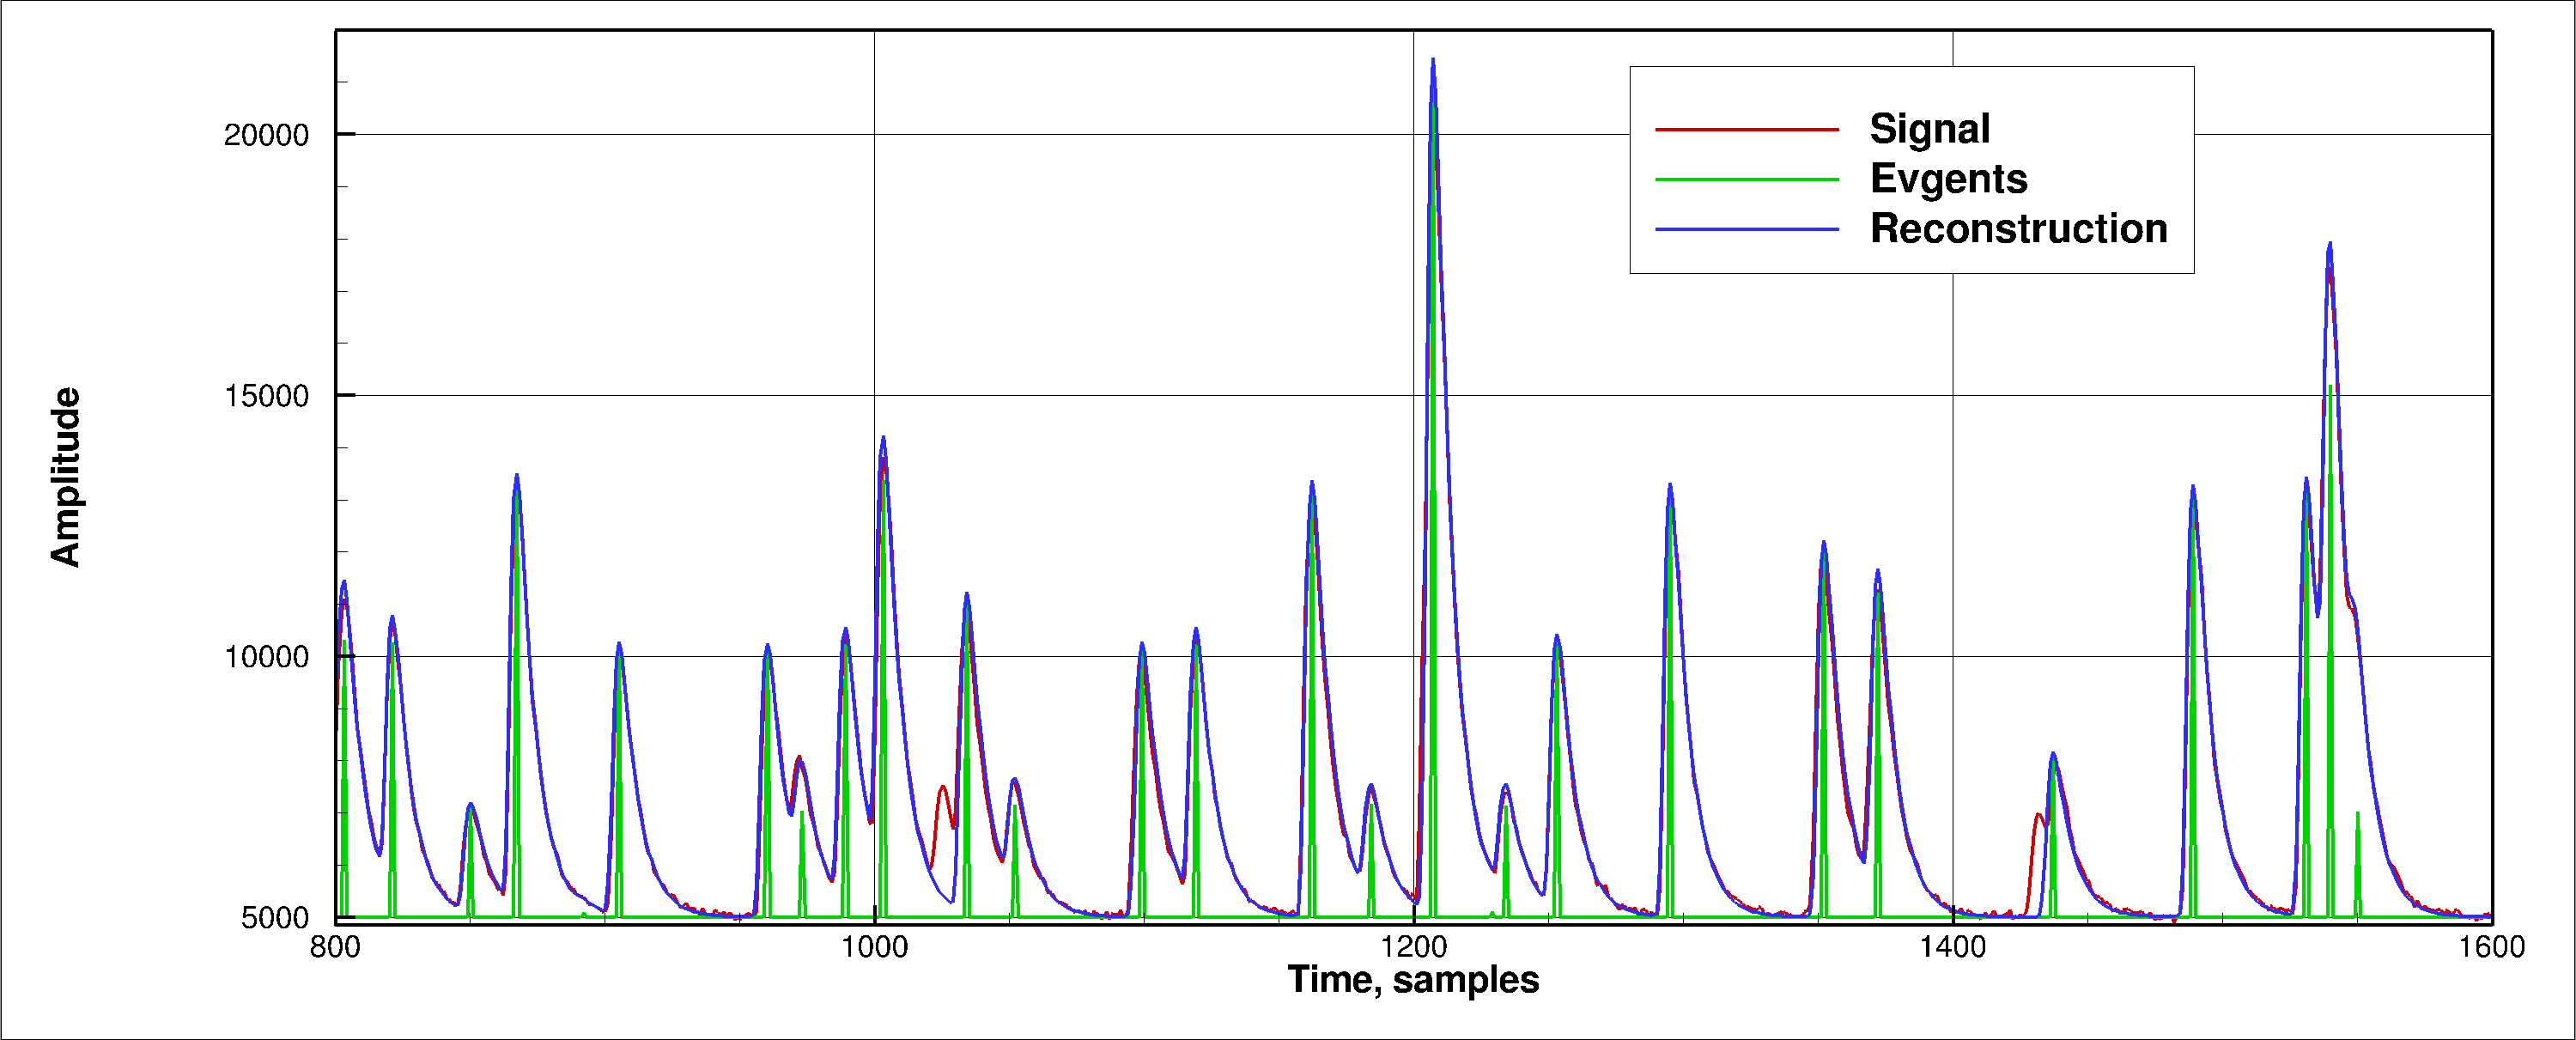
\includegraphics[width=0.95\linewidth]{deconvProcessing1e7} \\ а)
    \end{minipage}
    \vfill
    \begin{minipage}[b][][b]{0.95\linewidth}\centering
        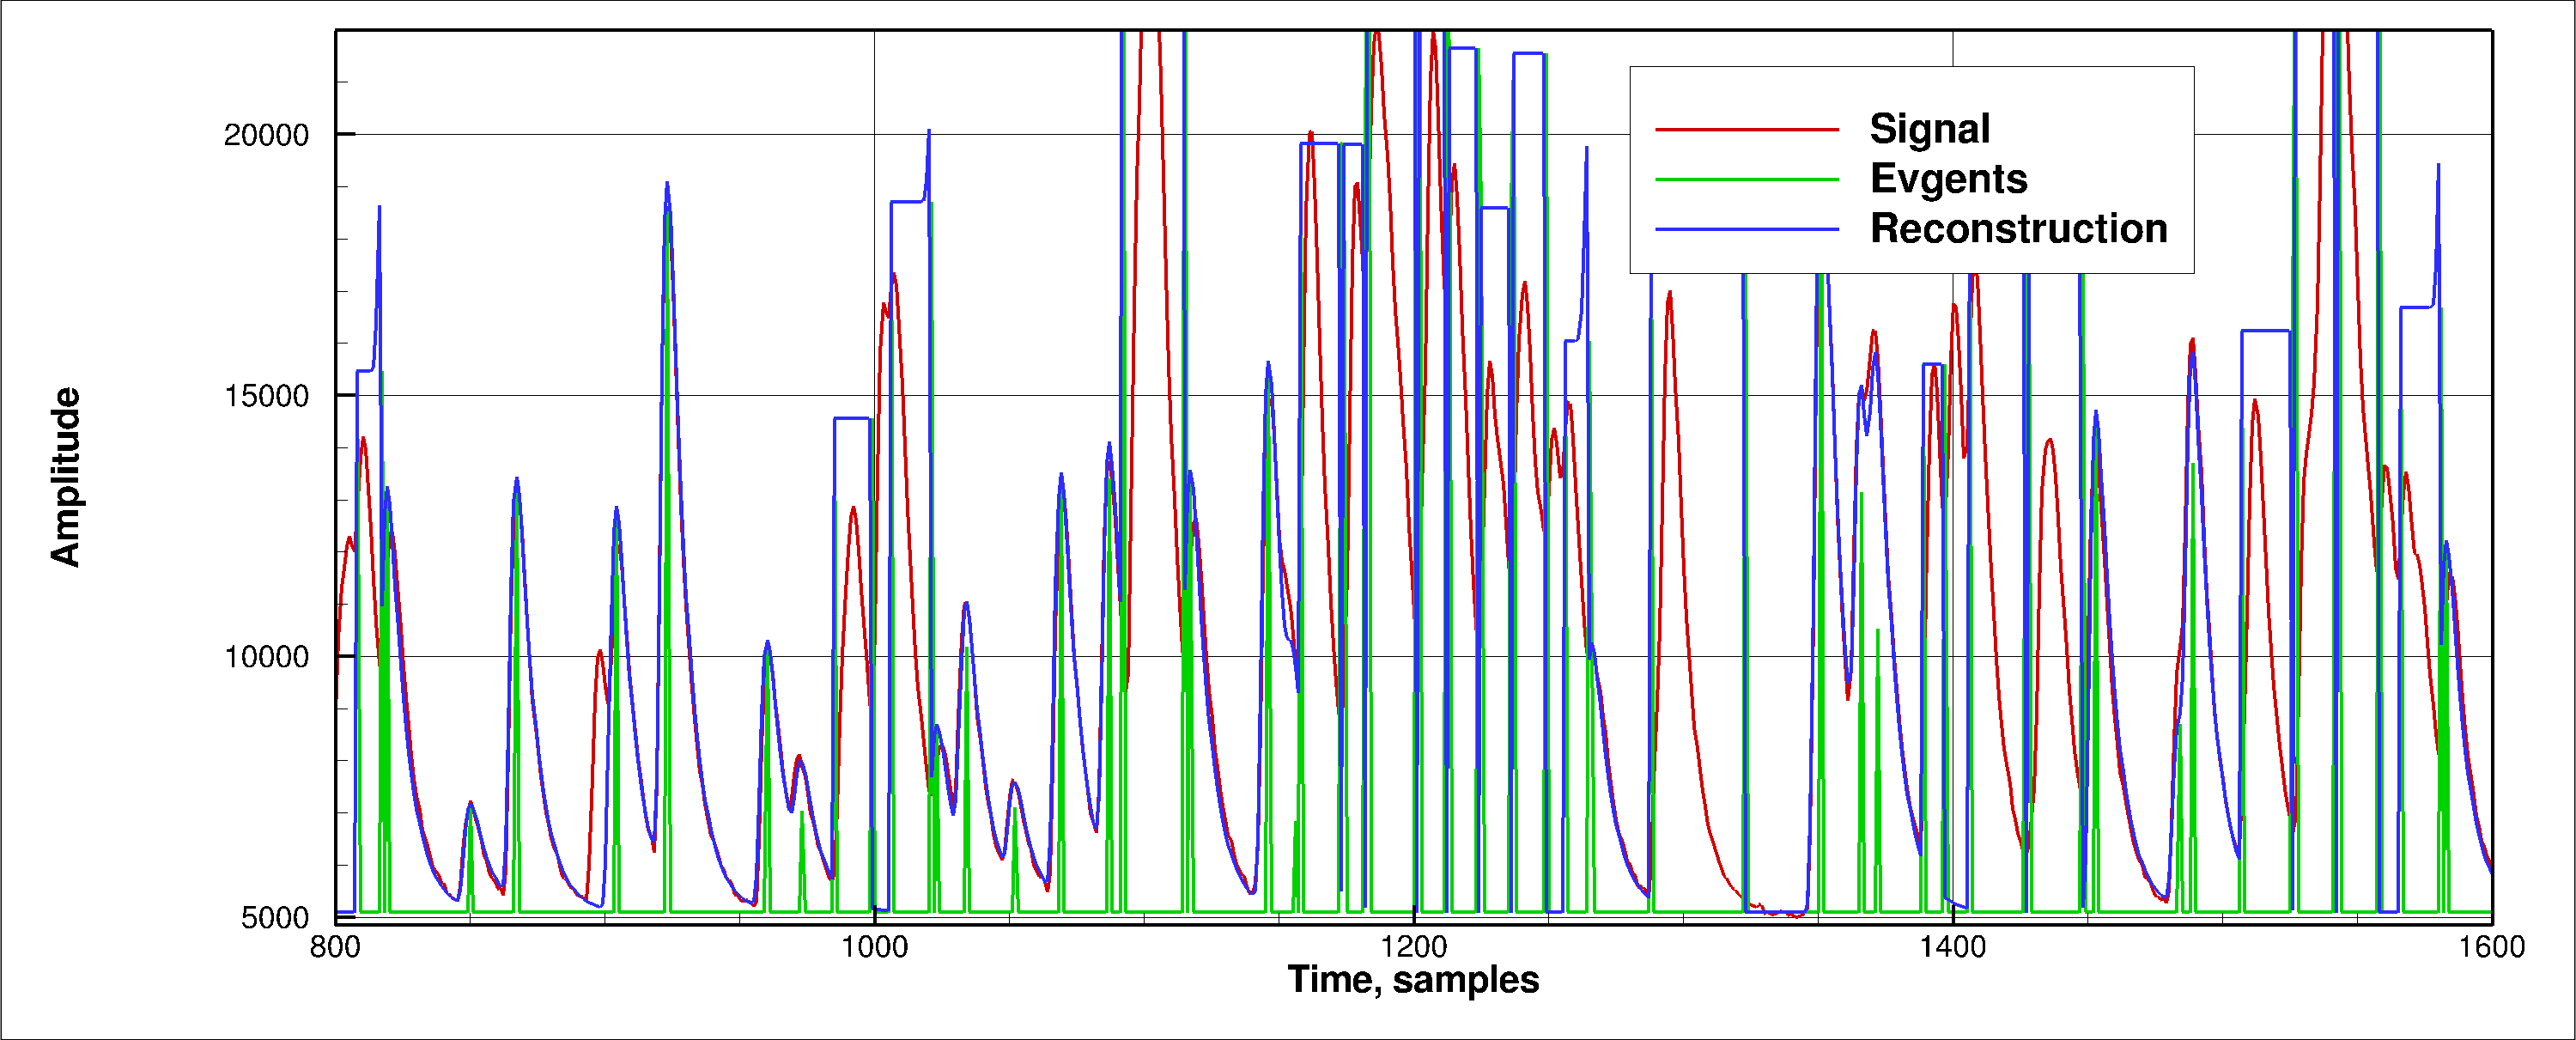
\includegraphics[width=0.95\linewidth]{deconvProcessing3e7} \\ б)
    \end{minipage}
    \vspace{5mm}
    \caption{ Пример работы алгоритма при обработке сигнала с загрузкой $10^7$~с${}^{-1}$~(а) и $3 \times 10^7$~с${}^{-1}$~(б). Красной линией обозначен модельный сигнал. Зелёным показан результат обработки сигнала с помощью алгоритма: импульсы, для которых $R/(E-B)<R^{max}$ и которые считаются успешно разобранными, представлены в виде единичных импульсов, а для импульсов, где $R/(E-B)>R^{max}$, на рисунке нарисован прямоугольник. Синим показан результат операции $z + \sum A_j p(t - t_j)$, то есть это такой сигнал, который соответствует разобранным импульсам; аналогично, для неразрешённых импульсов нарисован прямоугольник.~\cite{Khilkevitch2020}. }
    \label{fig:DeconvProcessing}
\end{figure}

% ----------------------------------------------------------

\subsection{Сравнение методов обрабоки сигнала}

Сравнение методов, описанных выше, для различных значений загрузки детектора, представлено на рисунках~\ref{fig:processingTotalCountRate},  \ref{fig:processingByWindowCountRate}, \ref{fig:processingByWindowFwhm}, \ref{fig:processingSpectrumCmpByMethods}, \ref{fig:processingSpectrumCmpByCountRate}. 

\begin{figure}[ht!]
  \centerfloat{ 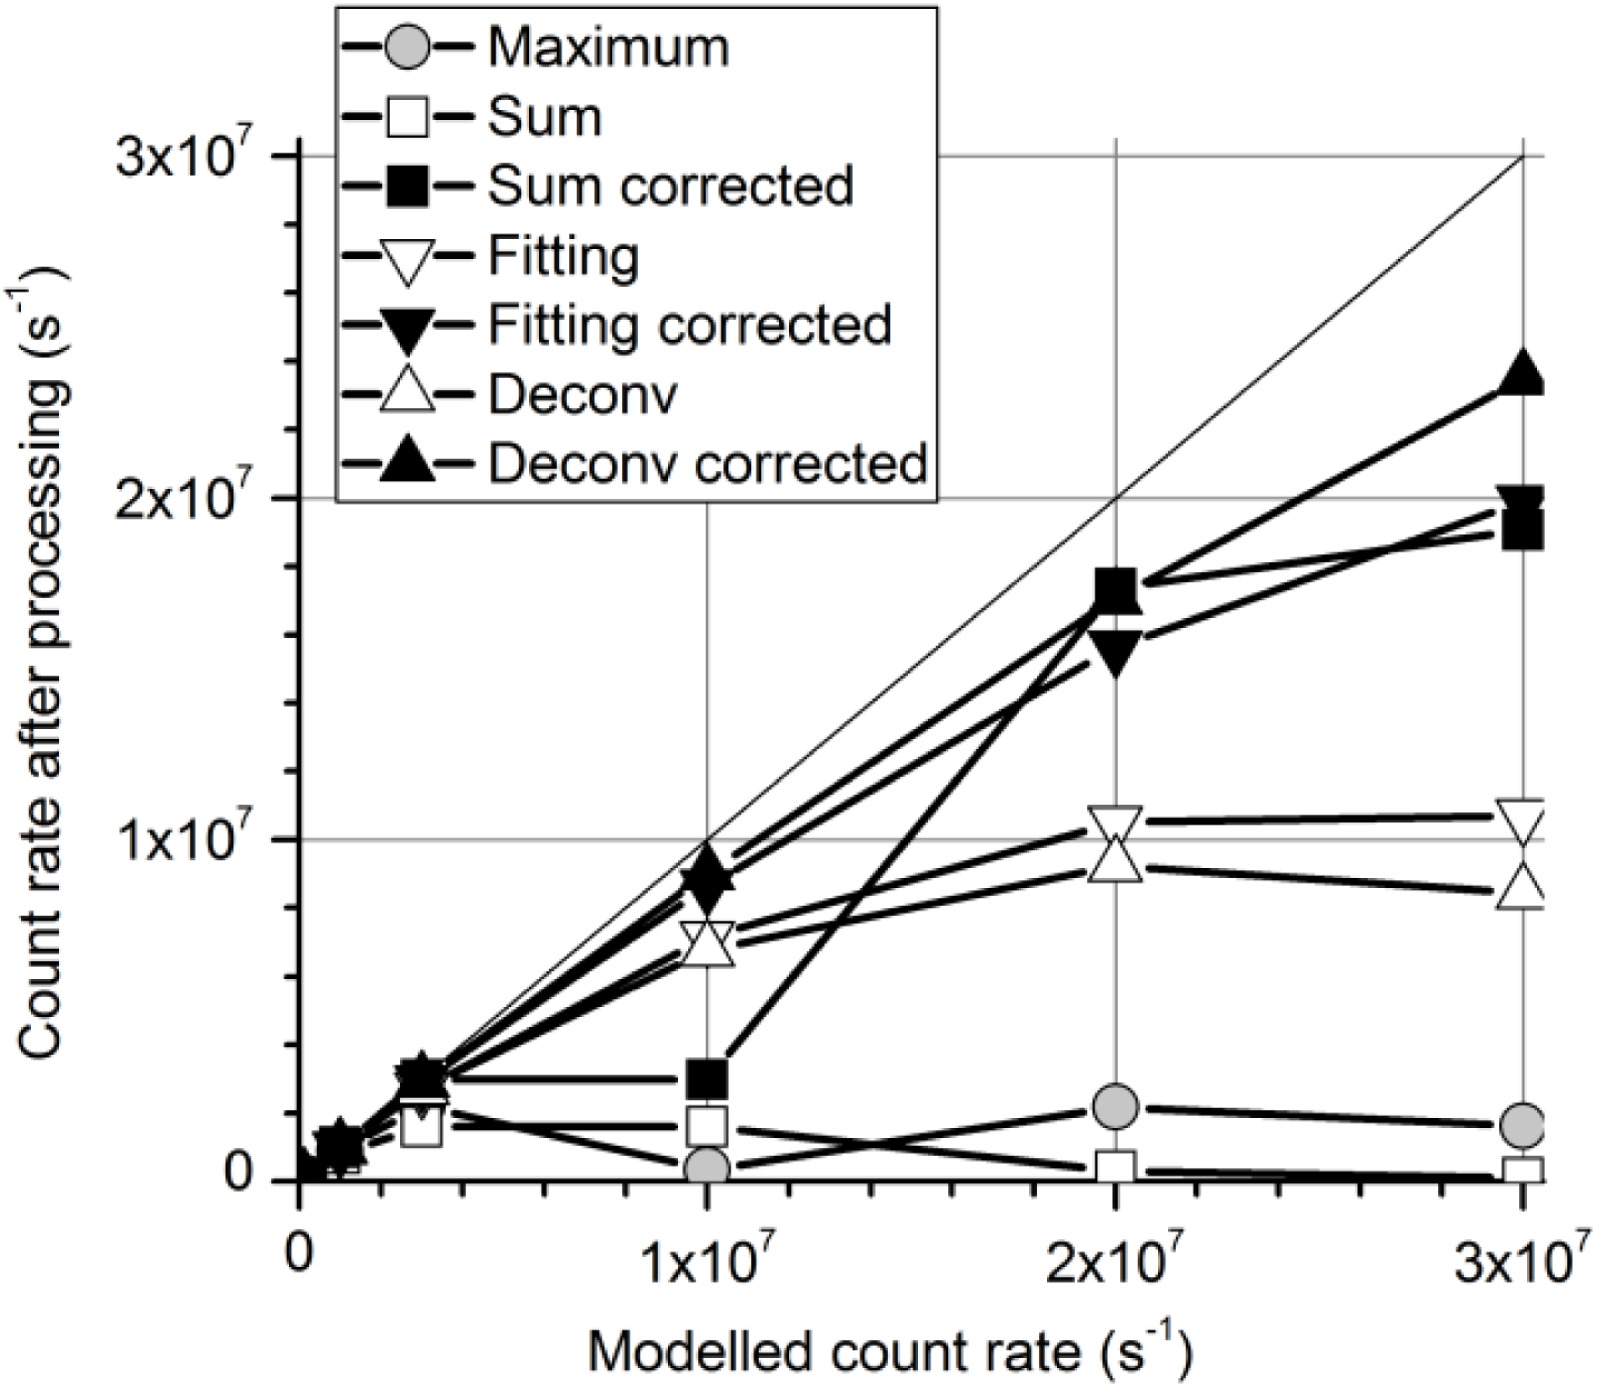
\includegraphics[width=0.60\linewidth]{processingTotalCountRate} }
  \caption{Общее количество зарегистрированных событий с энергиями выше 1~МэВ. В идеальном случае количество обнаруженных событий должно совпадать с количеством сгенерированных событий (сплошная линия). Однако из-за наложений во время обработки обнаруживается меньшее количество событий.~\cite{Khilkevitch2020} }
  \label{fig:processingTotalCountRate}
\end{figure}

\begin{figure}[ht!]
  \centerfloat{ 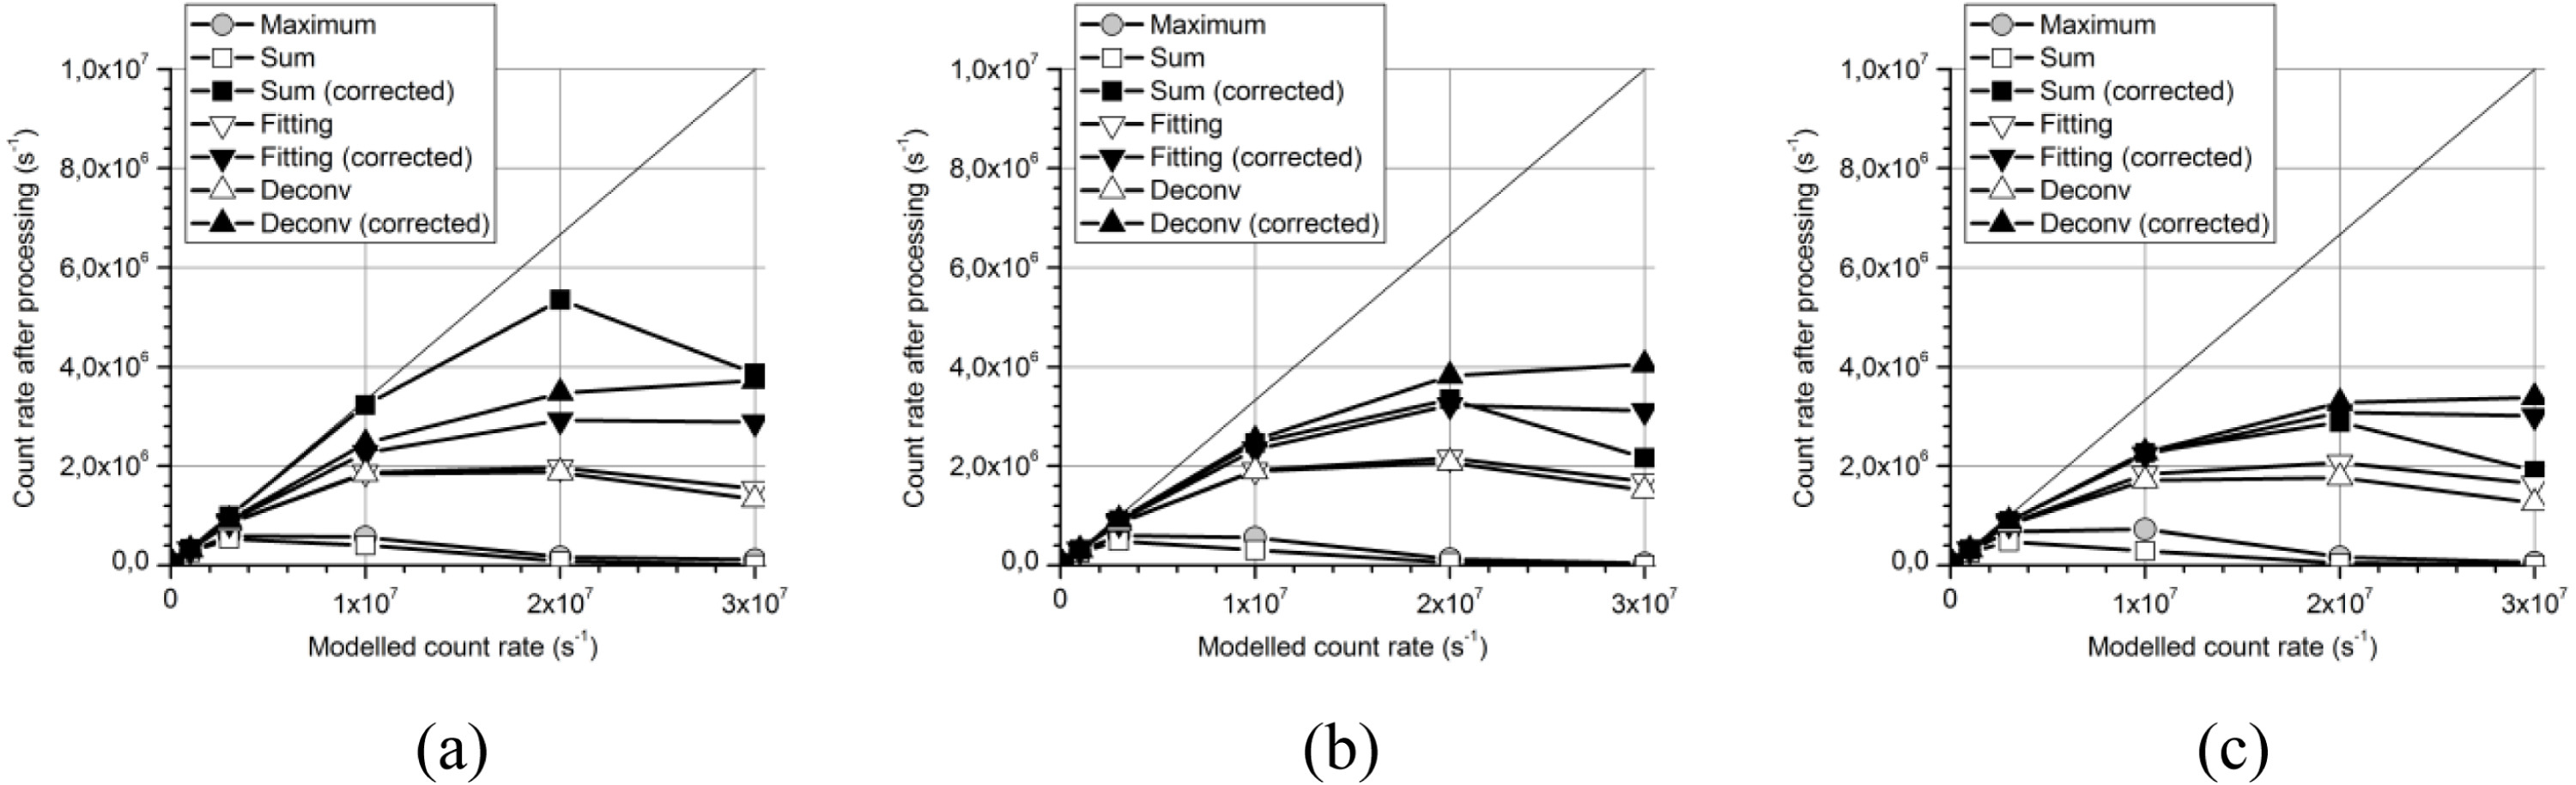
\includegraphics[width=0.95\linewidth]{processingByWindowCountRate} }
  \caption{ Количество событий в пиках с энергиями 2~МэВ~(а), 5~МэВ~(b) и 8~МэВ~(c) (в окне шириной 1~МэВ), полученных с использованием различных алгоритмов обработки. В идеальном случае количество обнаруженных событий должно быть равно одной трети количества сгенерированных событий (сплошные линии).~\cite{Khilkevitch2020} }
  \label{fig:processingByWindowCountRate}
\end{figure}

\begin{figure}[ht!]
  \centerfloat{ 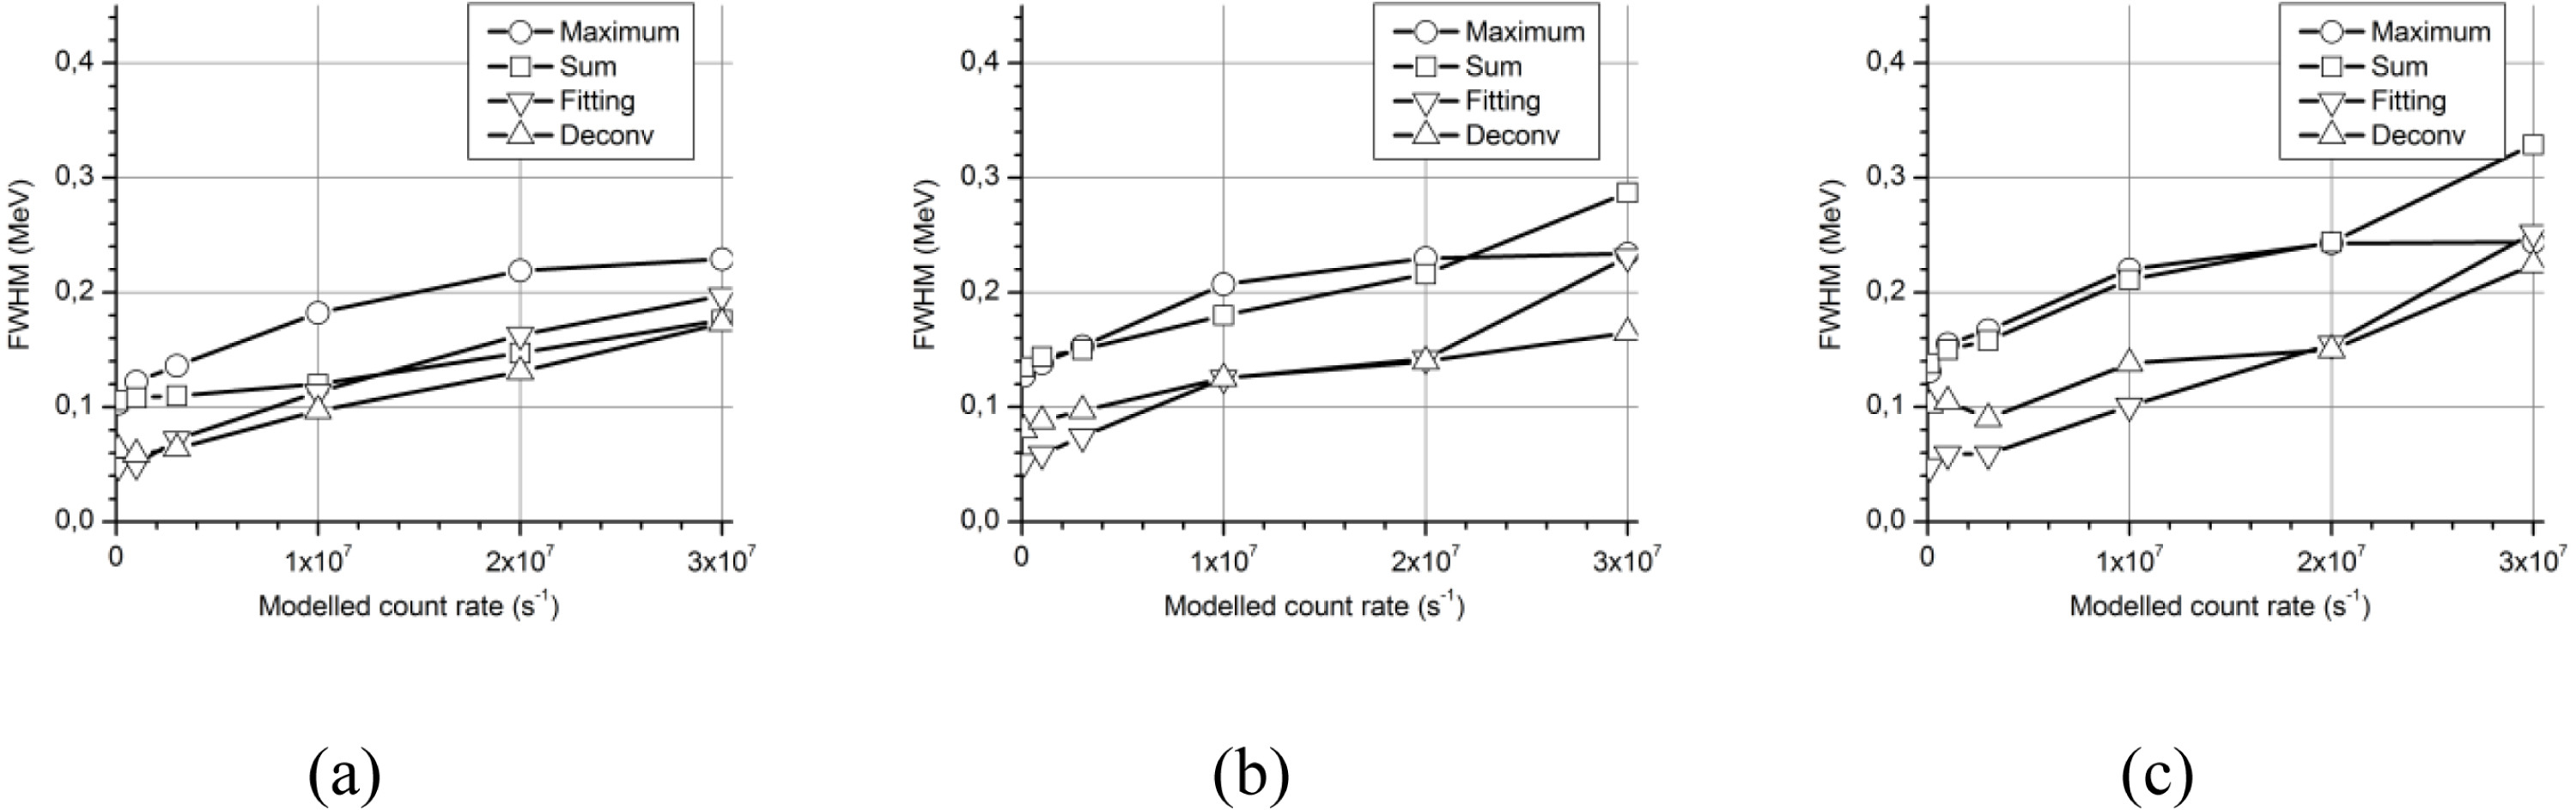
\includegraphics[width=0.95\linewidth]{processingByWindowFwhm} }
  \caption{ Полная ширина на полувысоте (FWHM) пиков при разных энергиях: 2~МэВ~(а), 5~МэВ~(b), 8~МэВ~(c).~\cite{Khilkevitch2020} }
  \label{fig:processingByWindowFwhm}
\end{figure}

\begin{figure}[ht!]
  \centerfloat{ 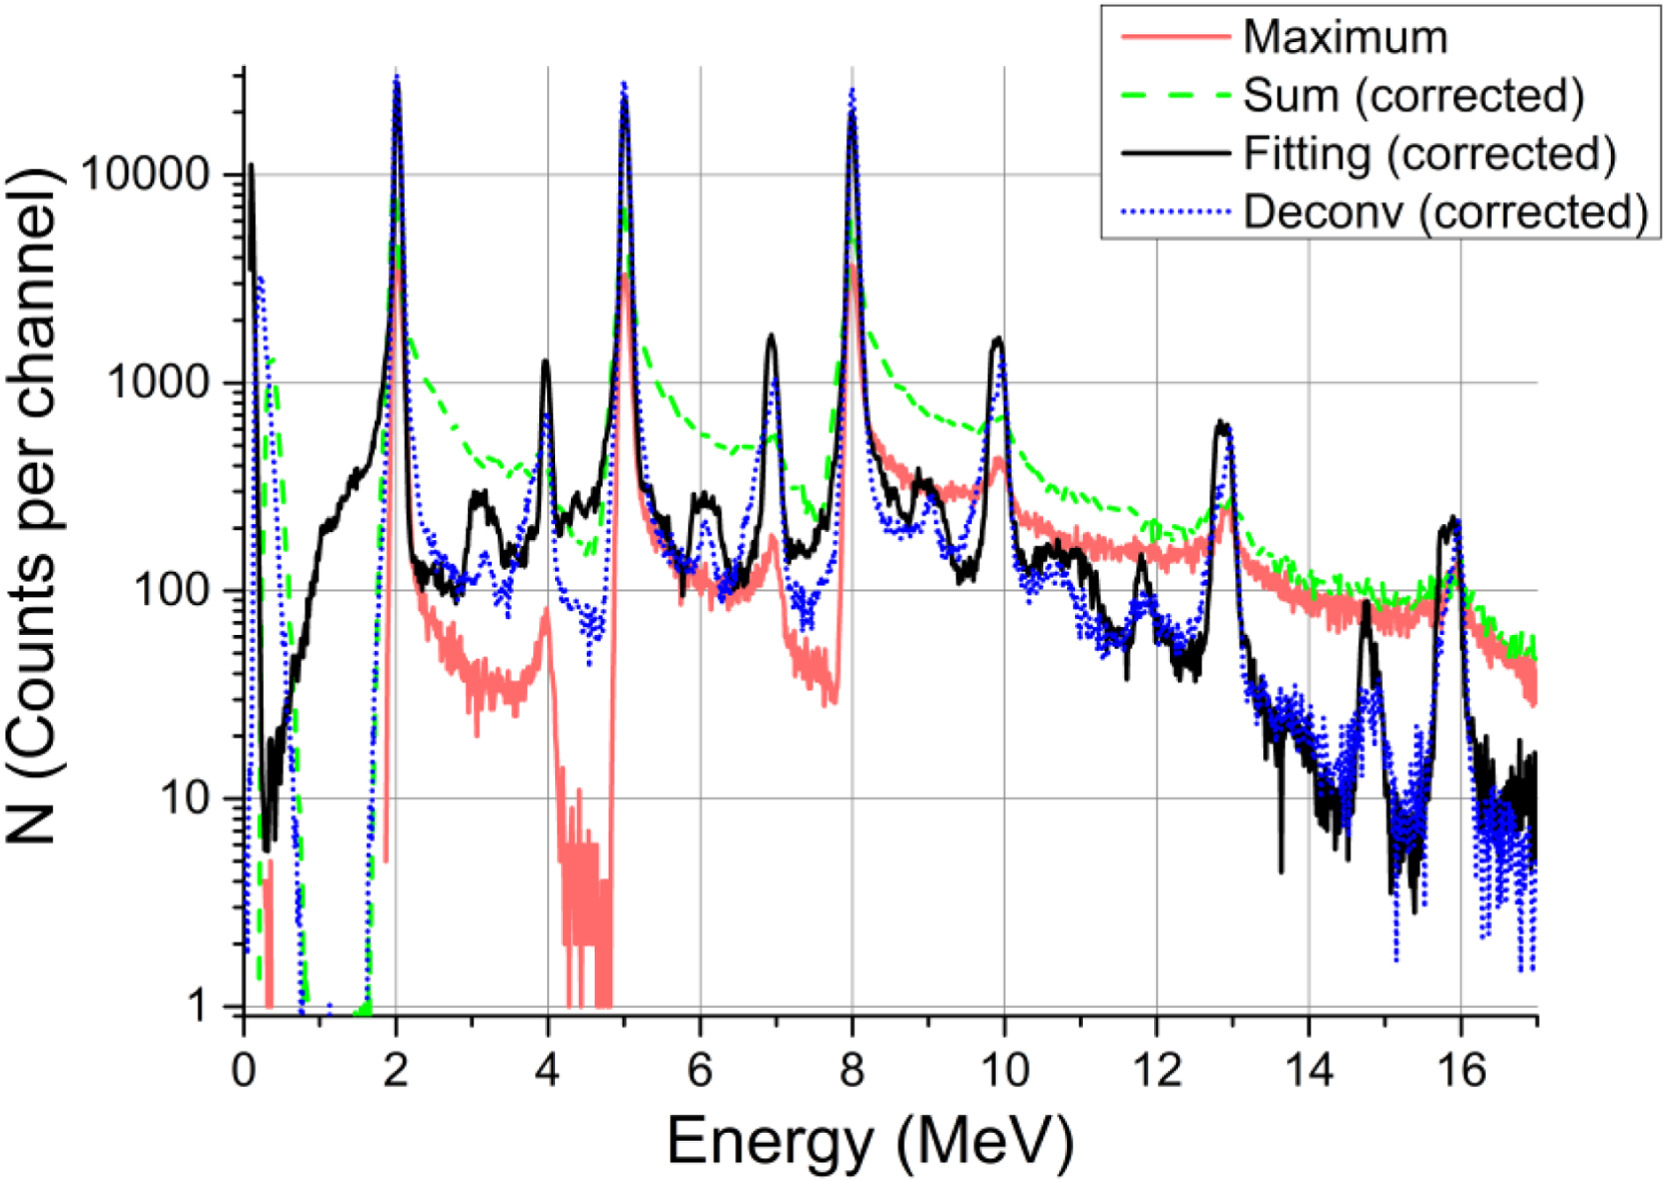
\includegraphics[width=0.60\linewidth]{processingSpectrumCmpByMethods} }
  \caption{ Спектры, полученные разными методами при загрузке детектора $10^7$~с${}^{-1}$. Спектры, полученные в ходе применения методов суммы, фиттигна и деконволюции показаны с коррекцией неразрешенных событий.~\cite{Khilkevitch2020} }
  \label{fig:processingSpectrumCmpByMethods}
\end{figure}

\begin{figure}[ht!]
  \centerfloat{ 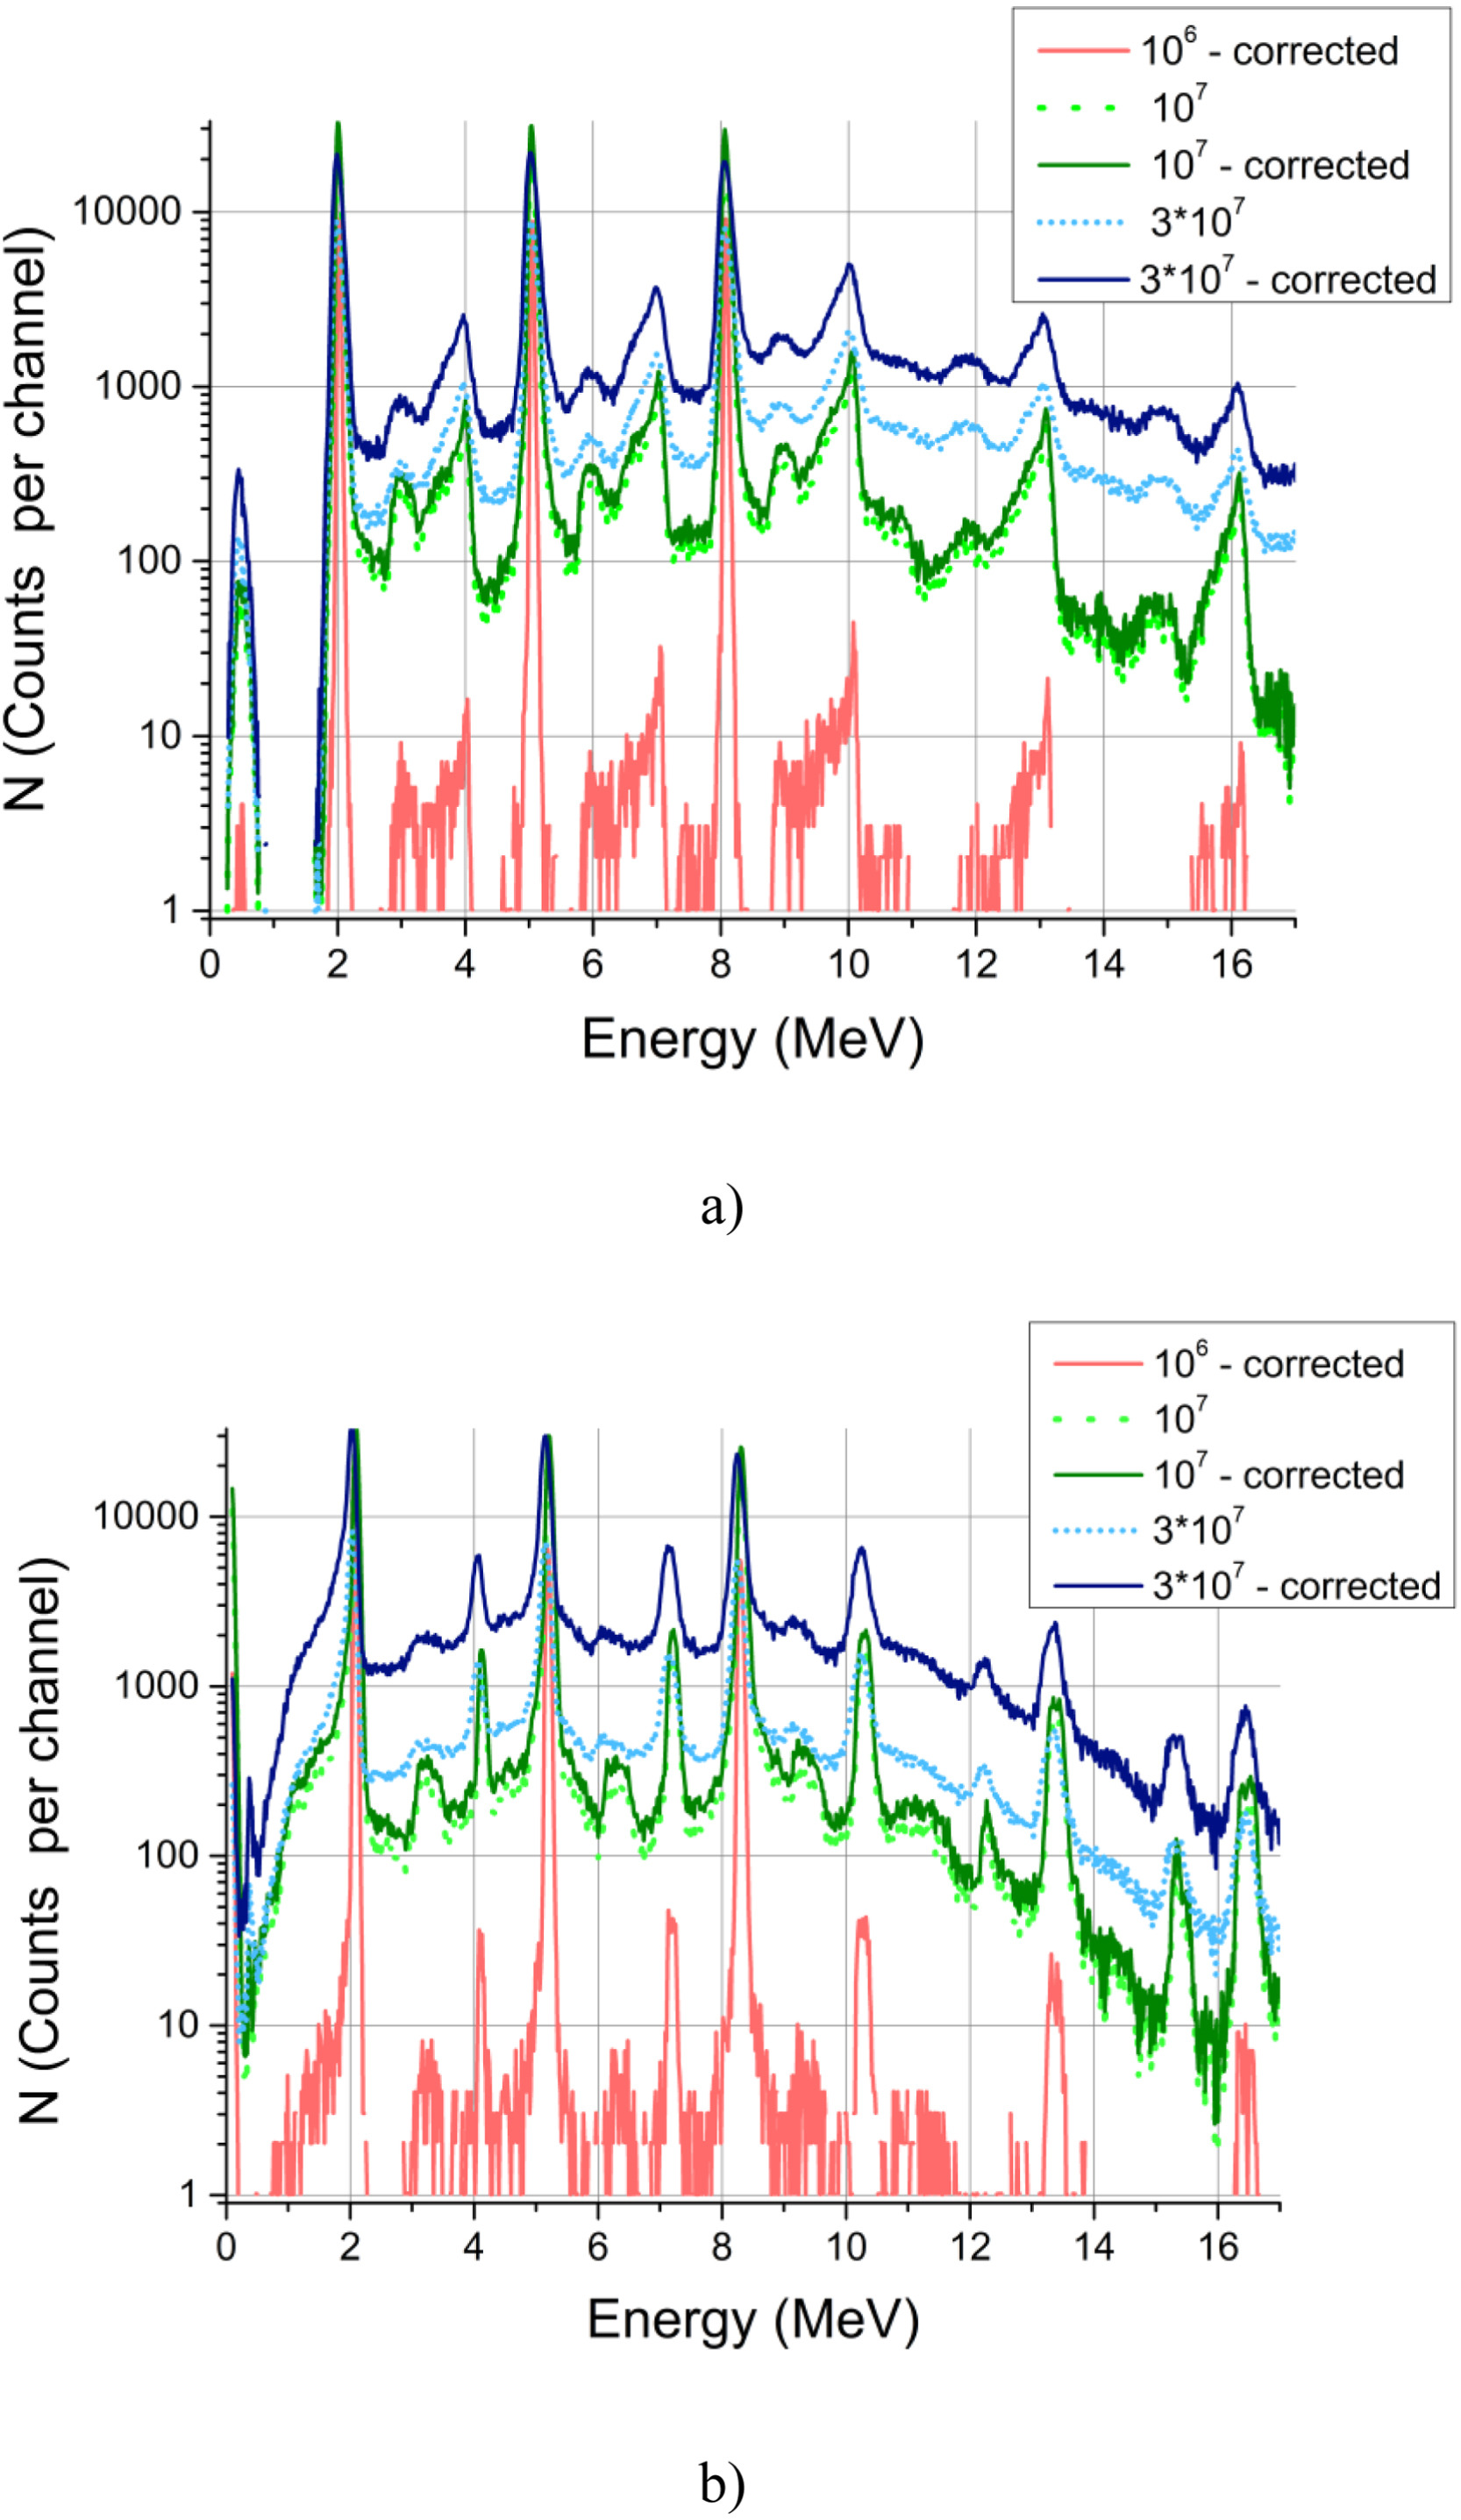
\includegraphics[width=0.60\linewidth]{processingSpectrumCmpByCountRate} }
  \caption{ Спектры, полученные методами фиттинга~(a) и деконволюции~(b). Линии, обозначенные как <<скорректированные>>, представляют собой спектры с коррекцией неразрешенных импульсов. При нагрузке $10^6$~с${}^{-1}$ спектры практически идентичны и их трудно различить на рисунках.~\cite{Khilkevitch2020} }
  \label{fig:processingSpectrumCmpByCountRate}
\end{figure}


Использованы модельные данные, созданные в разделе~\ref{sec:SignalGeneration}. На этих рисунках обозначения <<Sum corrected>>, <<Fitting corrected>> и <<Deconv corrected>> соответствуют данным, полученным с помощью алгоритмов <<суммы>>, <<фиттинга>> и <<деконволюции>> с учетом неразрешенных событий по ранее описанная процедуре. Эта поправка не влияет на форму результирующего спектра для стационарного источника излчения, как в модельном сигнале (однако, если спектр излучения меняется во времени, то это утверждение перестаёт быть верным). Однако такая коррекция позволяет получить более близкое к истинному количество событий, зарегистрированных детектором.

Использование метода <<максимум>> совершенно нецелесообразно при скоростях счета выше $3 \times 10^6$~с${}^{-1}$, так же как и использование метода <<суммы>> без коррекции неразрешённых событий из-за весьма высоких ошибок определения как общего числа событий, так и числа событий в одиночных пиках. Коррекция неразрешенных наложенных импульсов любым методом позволяет значительно улучшить результаты обработки сигнала. Наилучшие результаты определения числа импульсов в пиках дает метод деконволюции с коррекцией, дающий ошибку определения скорости счета при нагрузке $3 \times 10^7$~с${}^{-1}$ равной 21\%. Метод фиттинга с коррекцией менее точен, он дает погрешность скорости счета 33\% при той же нагрузке. Эта ошибка коррекции, по-видимому, увеличивается из-за роста количества слишком близких друг к другу импульсов, что приводит к тому, что они распознаются как одиночный импульс суммарной амплитуды. Метод суммы позволяет хорошо определить общее количество импульсов после коррекции, но количество неразрешенных событий при использовании этого алгоритма чрезвычайно велико при высоких нагрузках, что затрудняет его использование при измерении гамма-излучения высокотемпературной плазмы токамака, в котором спектр может значительно изменяться за короткие промежутки времени.

При определении интенсивностей отдельных пиков картина меняется. Погрешность определения интенсивности одиночных пиков при нагрузке свыше $10^7$~с${}^{-1}$ быстро возрастает. Это можно объяснить тем, что, хотя методы позволяют разделить наложенные импульсы, ошибки в определении их амплитуды становятся очень значительными для всех алгоритмов.

На рисунке~\ref{fig:processingByWindowFwhm} показано разрешение (полная ширина на полувысоте, FWHM) пиков с энергиями 2~МэВ, 5~МэВ и 8~МэВ с при обработке сигнала различными алгоритмами. Алгоритмы фиттинга и деконволюции позволяют получить разрешение отдельных пиков намного лучше, чем алгоритмы максимума и суммы. Алгоритм деконволюции несколько лучше алгоритма фиттинга при высоких значениях нагрузки ($2 \times 10^7$~с${}^{-1}$ и выше) и немного хуже при низких значениях нагрузки. По-видимому, это связано с тем, что данный алгоритм вносит дополнительную погрешность при учете событий, время регистрации которых находится между соседними отсчетами АЦП. Однако этот алгоритм позволяет лучше разделять очень близко наложенные друг на друга события, что важно при высокой загрузке детектора. При высоких нагрузках  алгоритм <<по максимуму>> имеет разрешение, сравнимое с более сложными алгоритмами; однако, принимая во внимание тот факт, что при такой нагрузке он позволяет регистрировать лишь около 5\% всех событий, трудно говорить о его применимости для таких нагрузок детекторов.

Спектры, построенные с использованием различных методов определения амплитуды импульса, представлены на рисунках~\ref{fig:processingSpectrumCmpByMethods} и \ref{fig:processingSpectrumCmpByCountRate}. На спектрах различимы пики с энергиями 4~МэВ, 7~МэВ и 10~МэВ, тогда как в исходном сигнале были сгенерированы только пики с энергиями 2~МэВ~, 5~МэВ, 8~МэВ. Пики появляются из-за очень близко наложенных событий, которые не могут быть разрешены с помощью алгоритмов. Такие пики практически неотличимы от единичного события с амплитудой, равной сумме этих событий. Видны пики с энергией 4~МэВ (сумма двух событий с энергией 2~МэВ), 7~МэВ (сумма двух событий с энергией 2~МэВ и 5~МэВ), 10~МэВ (сумма двух событий с энергией 5~МэВ или с энергиями 2~МэВ и 8~МэВ), 13~МэВ (сумма двух событий с энергиями 5~МэВ и 8~МэВ).

Форма и амплитуда пиков, полученные методами максимума и суммы, сильно искажаются даже при нагрузке $10^7$~с${}^{-1}$. Форма пиков в спектрах, построенных с помощью методов фиттинга и деконволюции, остаётся симметричной даже при загрузках до $3 \times 10^7$~с${}^{-1}$. Для такой загрузке метод деконволюции сохранил симметрию формы и для пиков, являющихся суммами событий. В стационарном источнике спектры с коррекцией отличаются от спектров без нее лишь постоянным множителем~\cite{Khilkevitch2020}.

% ----------------------------------------------------------

\subsection{Влияние шума на результаты обработки}

Для демонстрации влияния шума на результаты различных алгоритмов был сгенерирован дополнительный набор модельных сигналов с нагрузкой $10^7$~с${}^{-1}$ и различными значениями уровня шума $\sigma_n$ в диапазоне от 10 до 500. Остальные параметры сигнала такие же, как описано в разделе~\ref{sec:SignalGeneration}, включая калибровку. Эти тестовые сигналы обрабатывались с использованием различных алгоритмов. Влияние шума на результаты алгоритмов иллюстрируют рисунки~\ref{fig:processingNoiceByWindowCountRate}, \ref{fig:processingNoiceByWindowFwhm}, \ref{fig:processingSpectrumCmpByNoice}.

\begin{figure}[ht!]
  \centerfloat{ 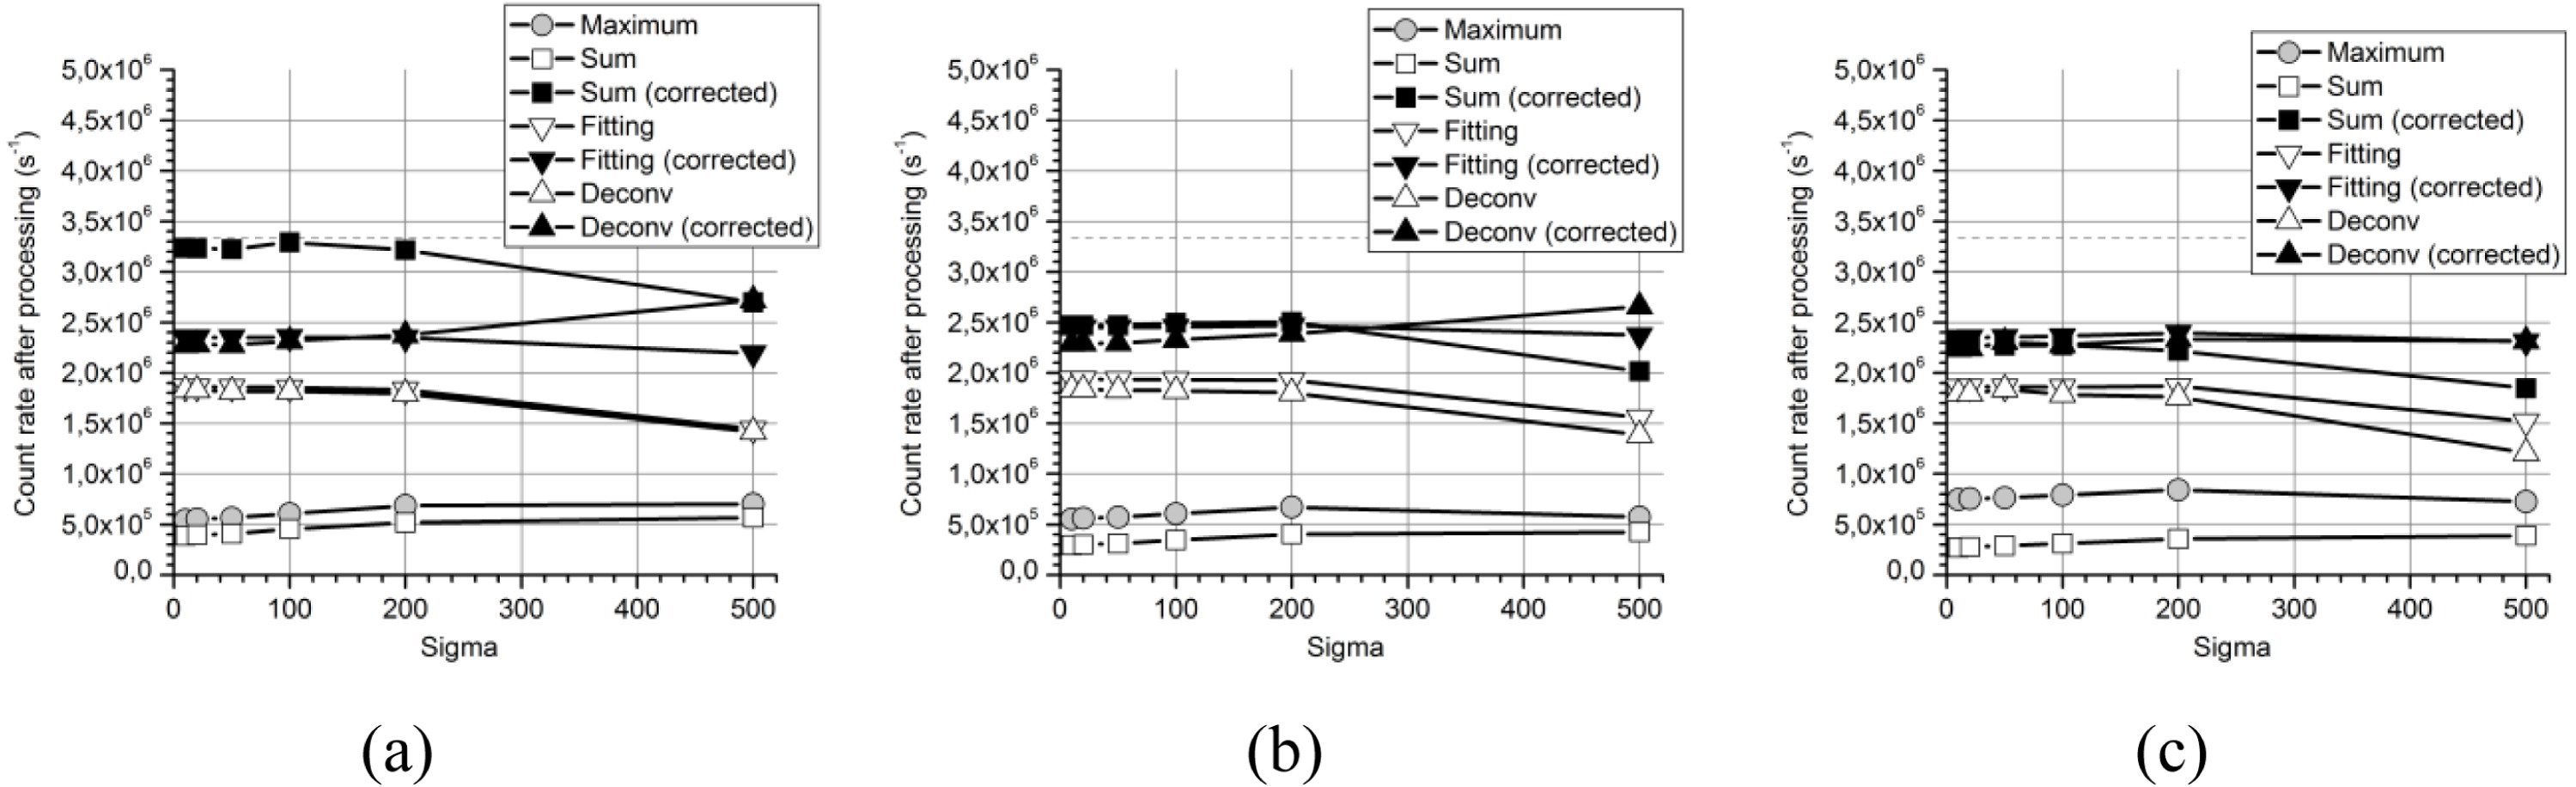
\includegraphics[width=0.95\linewidth]{processingNoiceByWindowCountRate} }
  \caption{ Количество событий в пиках с энергиями: 2~МэВ~(a), 5~МэВ~(b) и 8~МэВ~(c) (в окне шириной 1~МэВ), полученных с использованием различных алгоритмов обработки при разных значениях $\sigma_n$. Количество событий в идеальном случае равно $3.33 \times 10^6$.~\cite{Khilkevitch2020} }
  \label{fig:processingNoiceByWindowCountRate}
\end{figure}


\begin{figure}[ht!]
  \centerfloat{ 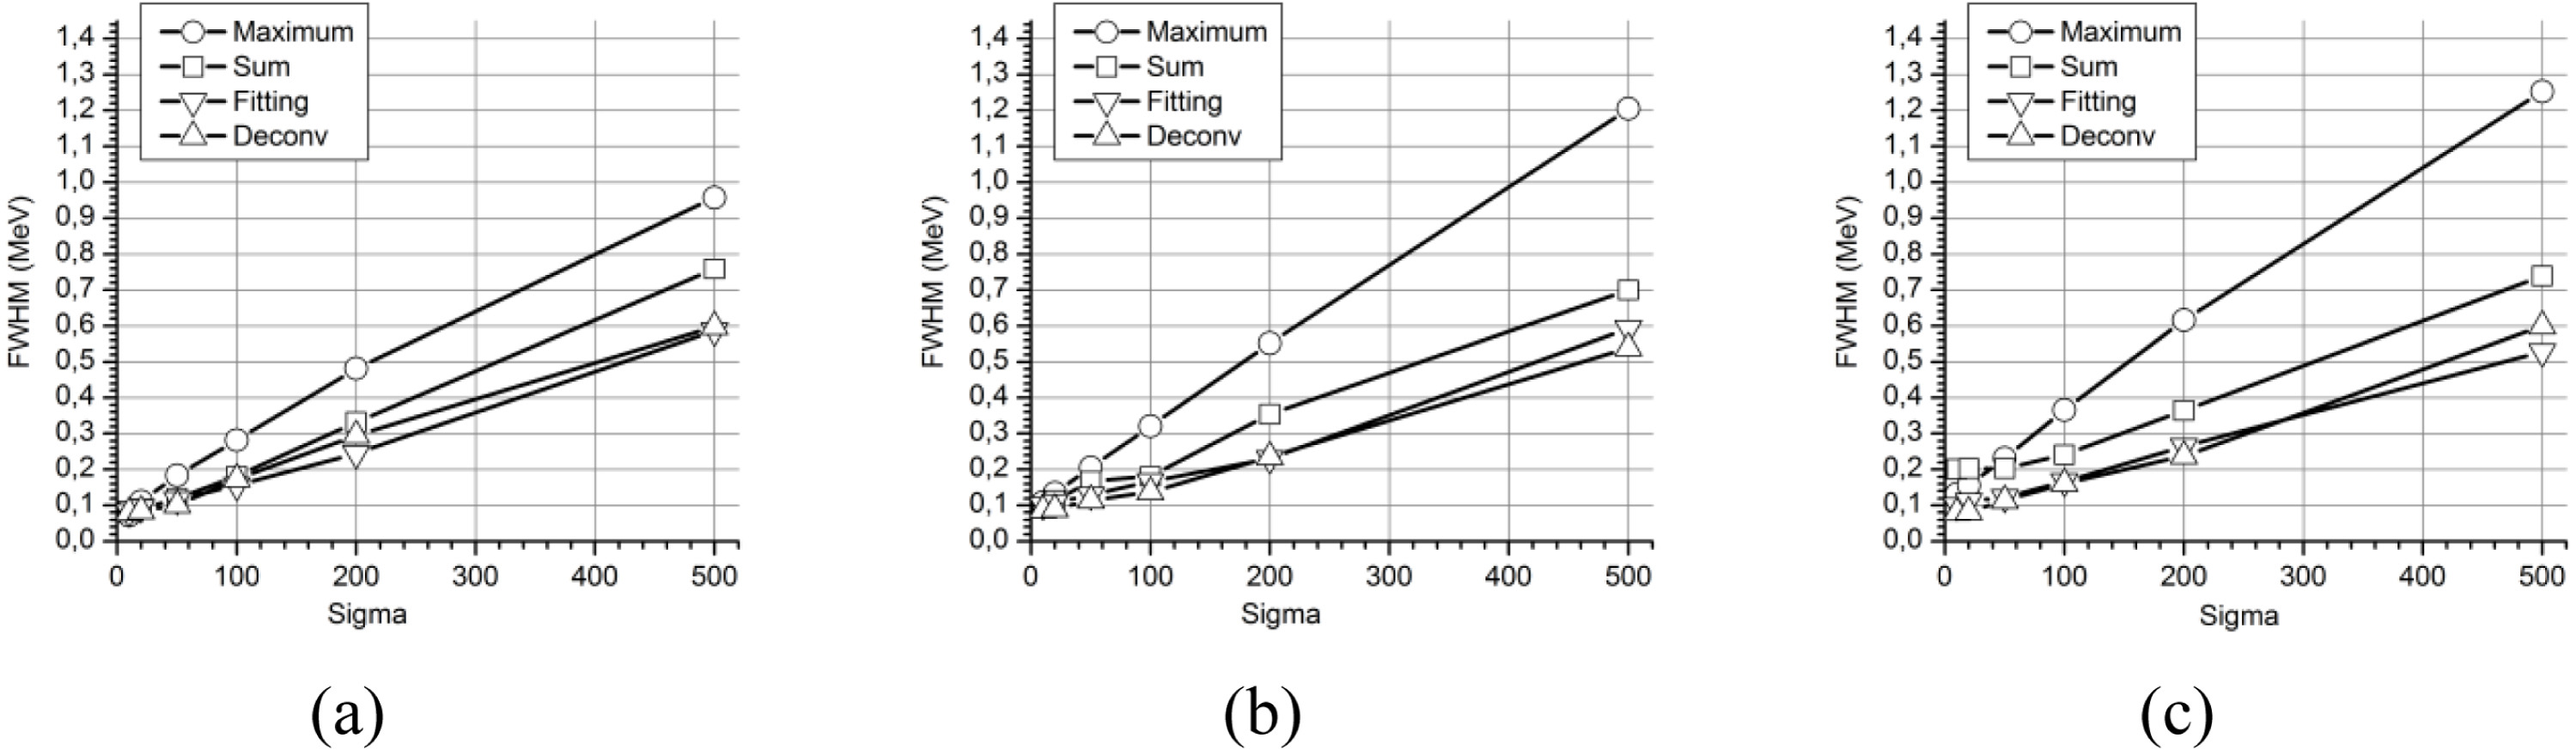
\includegraphics[width=0.95\linewidth]{processingNoiceByWindowFwhm} }
  \caption{ Полная ширина на полувысоте (FWHM) для пиков с энергиями: 2~МэВ~(a), 5~МэВ~(b) и 8~МэВ~(c), полученные с использованием различных алгоритмов обработки при разных значениях $\sigma_n$.~\cite{Khilkevitch2020} }
  \label{fig:processingNoiceByWindowFwhm}
\end{figure}

\begin{figure}[ht!]
  \centerfloat{ 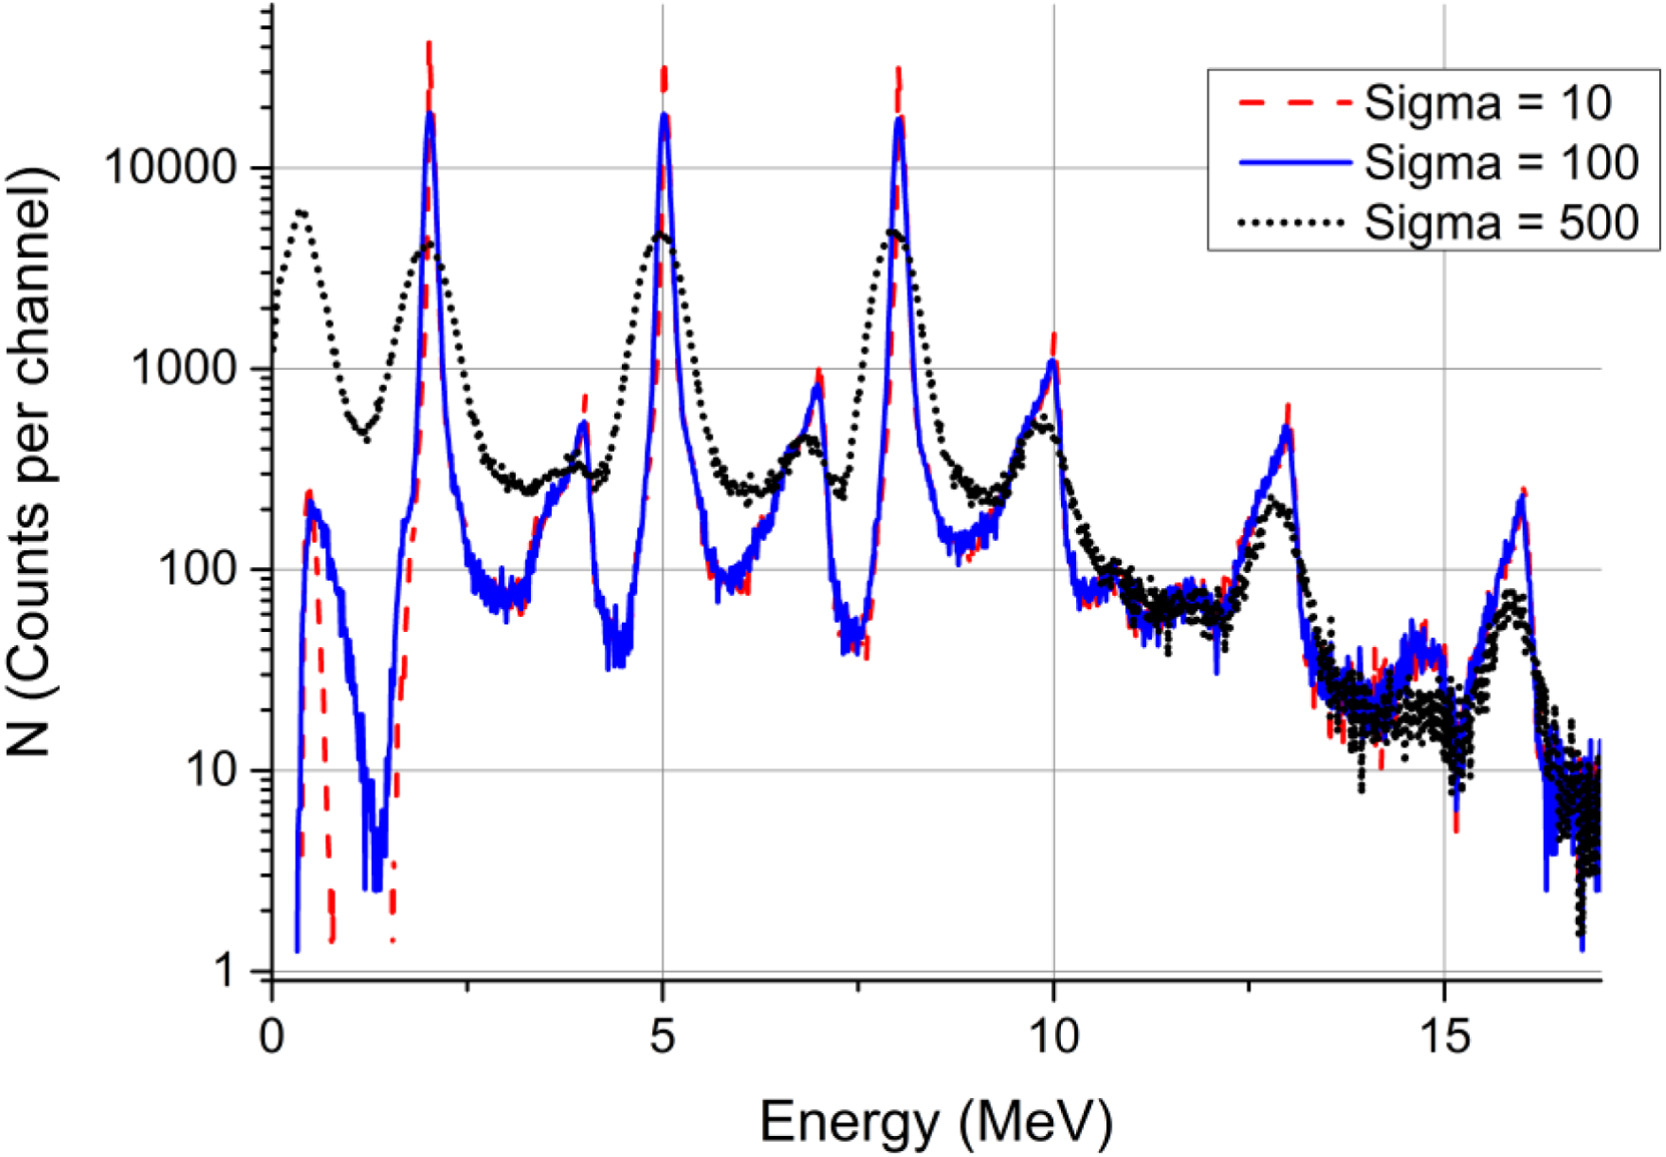
\includegraphics[width=0.65\linewidth]{processingSpectrumCmpByNoice} }
  \caption{ Спектры, полученные при обработке сигнала при нагрузке $10^7$~с${}^{-1}$ методом фиттинга с коррекцией спектра при различных значениях $\sigma_n$.~\cite{Khilkevitch2020} }
  \label{fig:processingSpectrumCmpByNoice}
\end{figure}


При уровне шума $\sigma_n \le 200$ количество отсчетов в пиках существенно не меняется при обработке любым из алгоритмов. При $\sigma_n = 500$ в отсутствие коррекции число событий на пиках, полученных при разделении импульсов, уменьшается. Это связано с тем, что ширина пика становится такой, что не все пиковые события попадают в энергетическое окно шириной 1~МэВ, как показано на рисунке~\ref{fig:processingSpectrumCmpByNoice}.

Полная ширина на полувысоте увеличивается в зависимости от уровня шума. При низких уровнях шума различия между алгоритмами практически несущественны. Однако при обработке алгоритмом <<по максимуму>> полуширина быстро линейно возрастает, что является очевидным свойством этого метода. Темпы роста ширины на полувысоте для спектров, полученных с помощью других алгоритмов, значительно ниже. Зависимость разрешения от уровня шума для спектров, полученных с помощью методов деконволюции и фиттинга, очень похожа.~\cite{Khilkevitch2020}

% ----------------------------------------------------------

\subsection{Время обработки сигнала}

Описанные выше алгоритмы имеют существенно разную алгоритмическую сложность. Время работы программы, в которой они были реализованы, зависит от конкретной программной реализации, аппаратной мощности компьютера, параметров обработки сигналов, а так же нагрузки детектора. Эти алгоритмы реализованы в компьютерном коде <<DeGaSum>>~\cite{Khilkevitch2020}. Код написан на языке программирования C++, а обработка происходит в несколько потоков с использованием SIMD-инструкций процессора.

\begin{figure}[ht!]
  \centerfloat{ 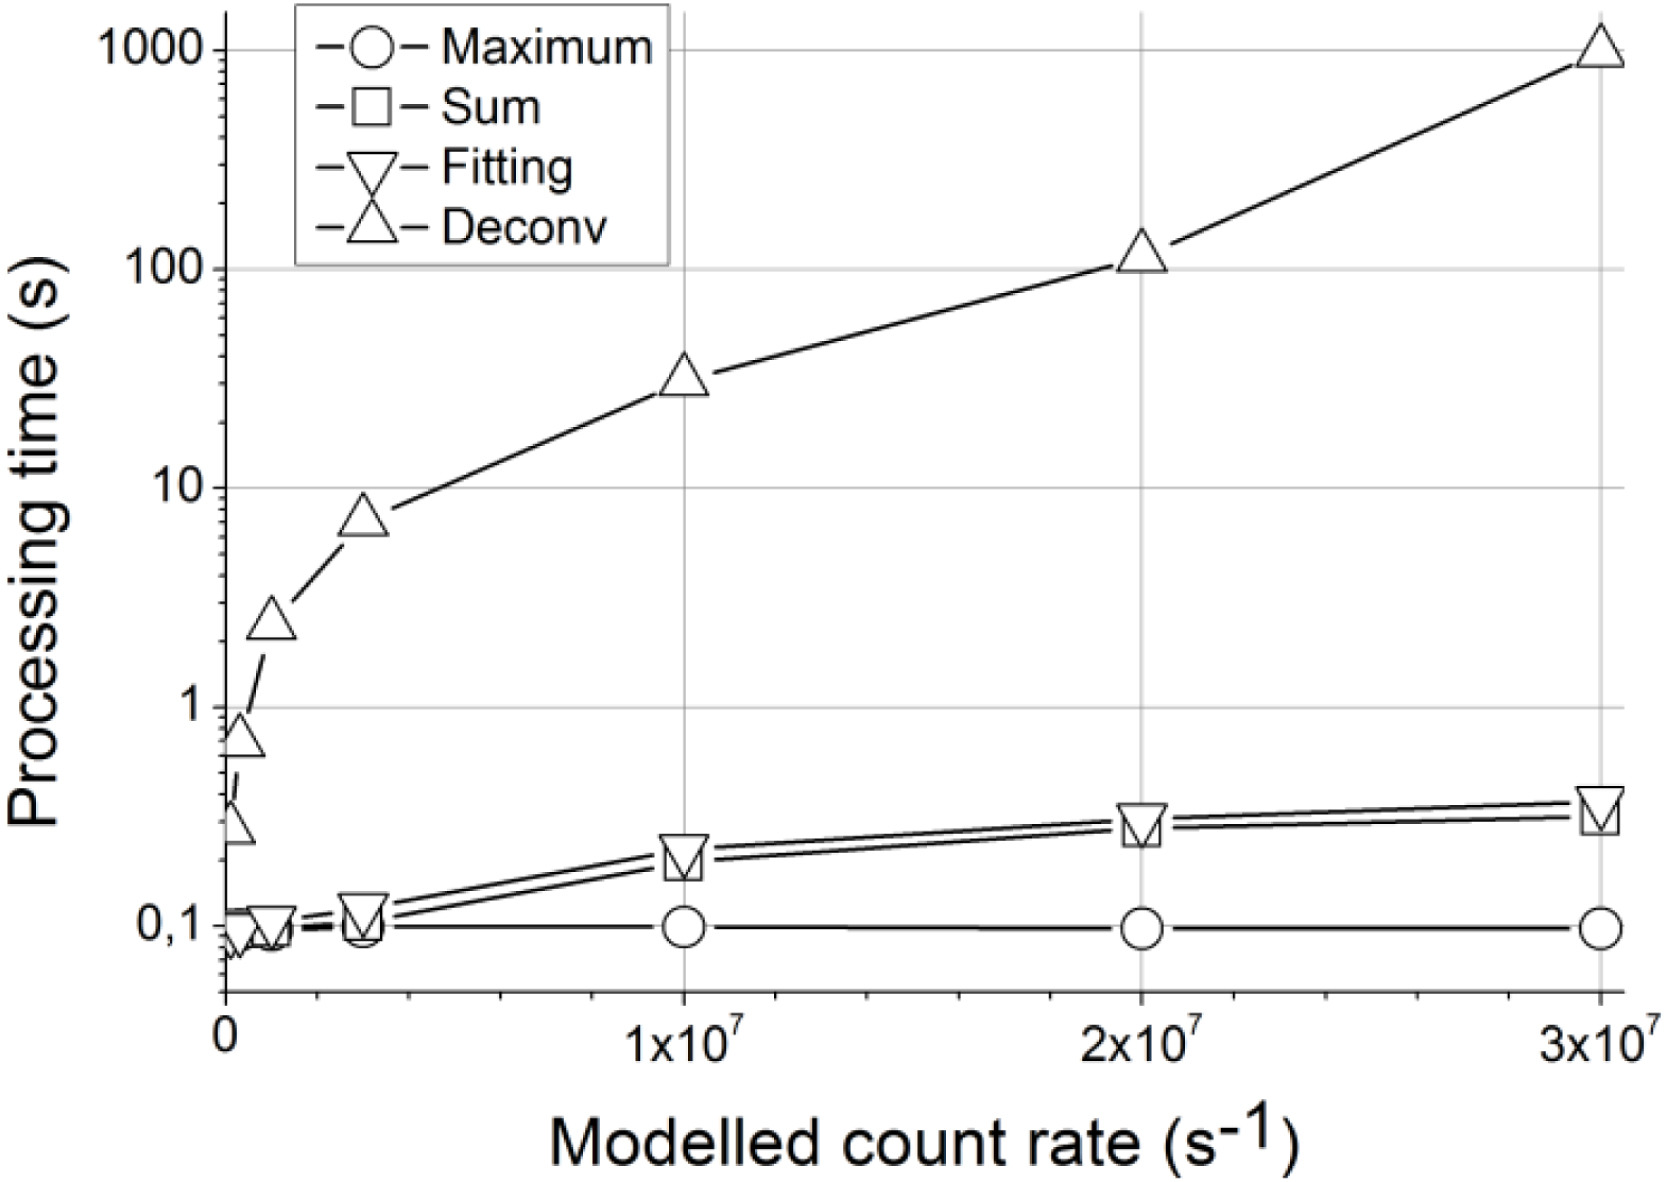
\includegraphics[width=0.65\linewidth]{processingTime} }
  \caption{ Время обработки смоделированного в разделе~\ref{sec:SignalGeneration} сигналов с использованием кода DeGaSum различными алгоритмами. В процессе обработки значение нулевой линии рассчитывалось по первым 10000 точкам сигнала. Модельный сигнал соответствуют длительности сбора данных 0.1~с при частоте дискретизации АЦП 250~МГц. Для обработки использовался ПК с процессором Intel Core i7-2700K@3.50~ГГц, 32~ГБ оперативной памяти, операционная система Debian Linux~10.4, код был скомпилирован с помощью g++~8.3.~\cite{Khilkevitch2020} }
  \label{fig:processingTime}
\end{figure}

На рисунке~\ref{fig:processingTime} показано время обработки модельного сигнала с использованием различных алгоритмов. Метод определения по максимум является простейшим вычислительным методом. Его производительность практически не зависит от загрузки детектора. Это связано с тем, что для его реализации необходим только последовательный поиск локальных максимумов. Другие методы требуют дополнительной обработки в областях, где значение сигнала превышает пороговый уровень, поэтому время их работы зависит от загрузки детектора. Метод деконволюции является наиболее затратным по вычислительным ресурсам, превосходя другие методы на порядки, особенно при больших нагрузках детектора. Это связано с тем, что его реализация требует дорогостоящих вычислительных операций для умножения матрицы и вектора.~\cite{Khilkevitch2020}

% ==========================================================

\section{Применение методов обработки на измеренных сигналах в экспериментах}

Для демонстрации работы алгоритмов был использован сигнал, полученный в ходе измерений, проведенных на циклотроне ФТИ им. А.Ф.~Иоффе~\cite{Lemberg1987}. Во время измерений пучок альфа-частиц направлялся на бериллиевую мишень, вызывая ядерную реакцию ${}^9Be(\alpha,n\gamma){}^{12}C$ с испусканием гамма-квантов с энергией 4,44~МэВ. Для измерений использовался сцинтилляционный детектор LaBr3(Ce) диаметром 76~мм с ФЭУ Hamamatsu R10233-100. Сигнал детектора оцифровывался с помощью платы АЦП ADP201X1/ADM214x400M/2A производства ЗАО <<Инструментальные системы>> с частотой дискретизации 250~МГц и записывался на жёсткий диск компьютера. Во время измерений менялся ток ионного пучка, что позволяло получать разные уровни загрузки детектора. Циклотрон работал в импульсном режиме.

\begin{figure}[ht!]
  \centerfloat{ 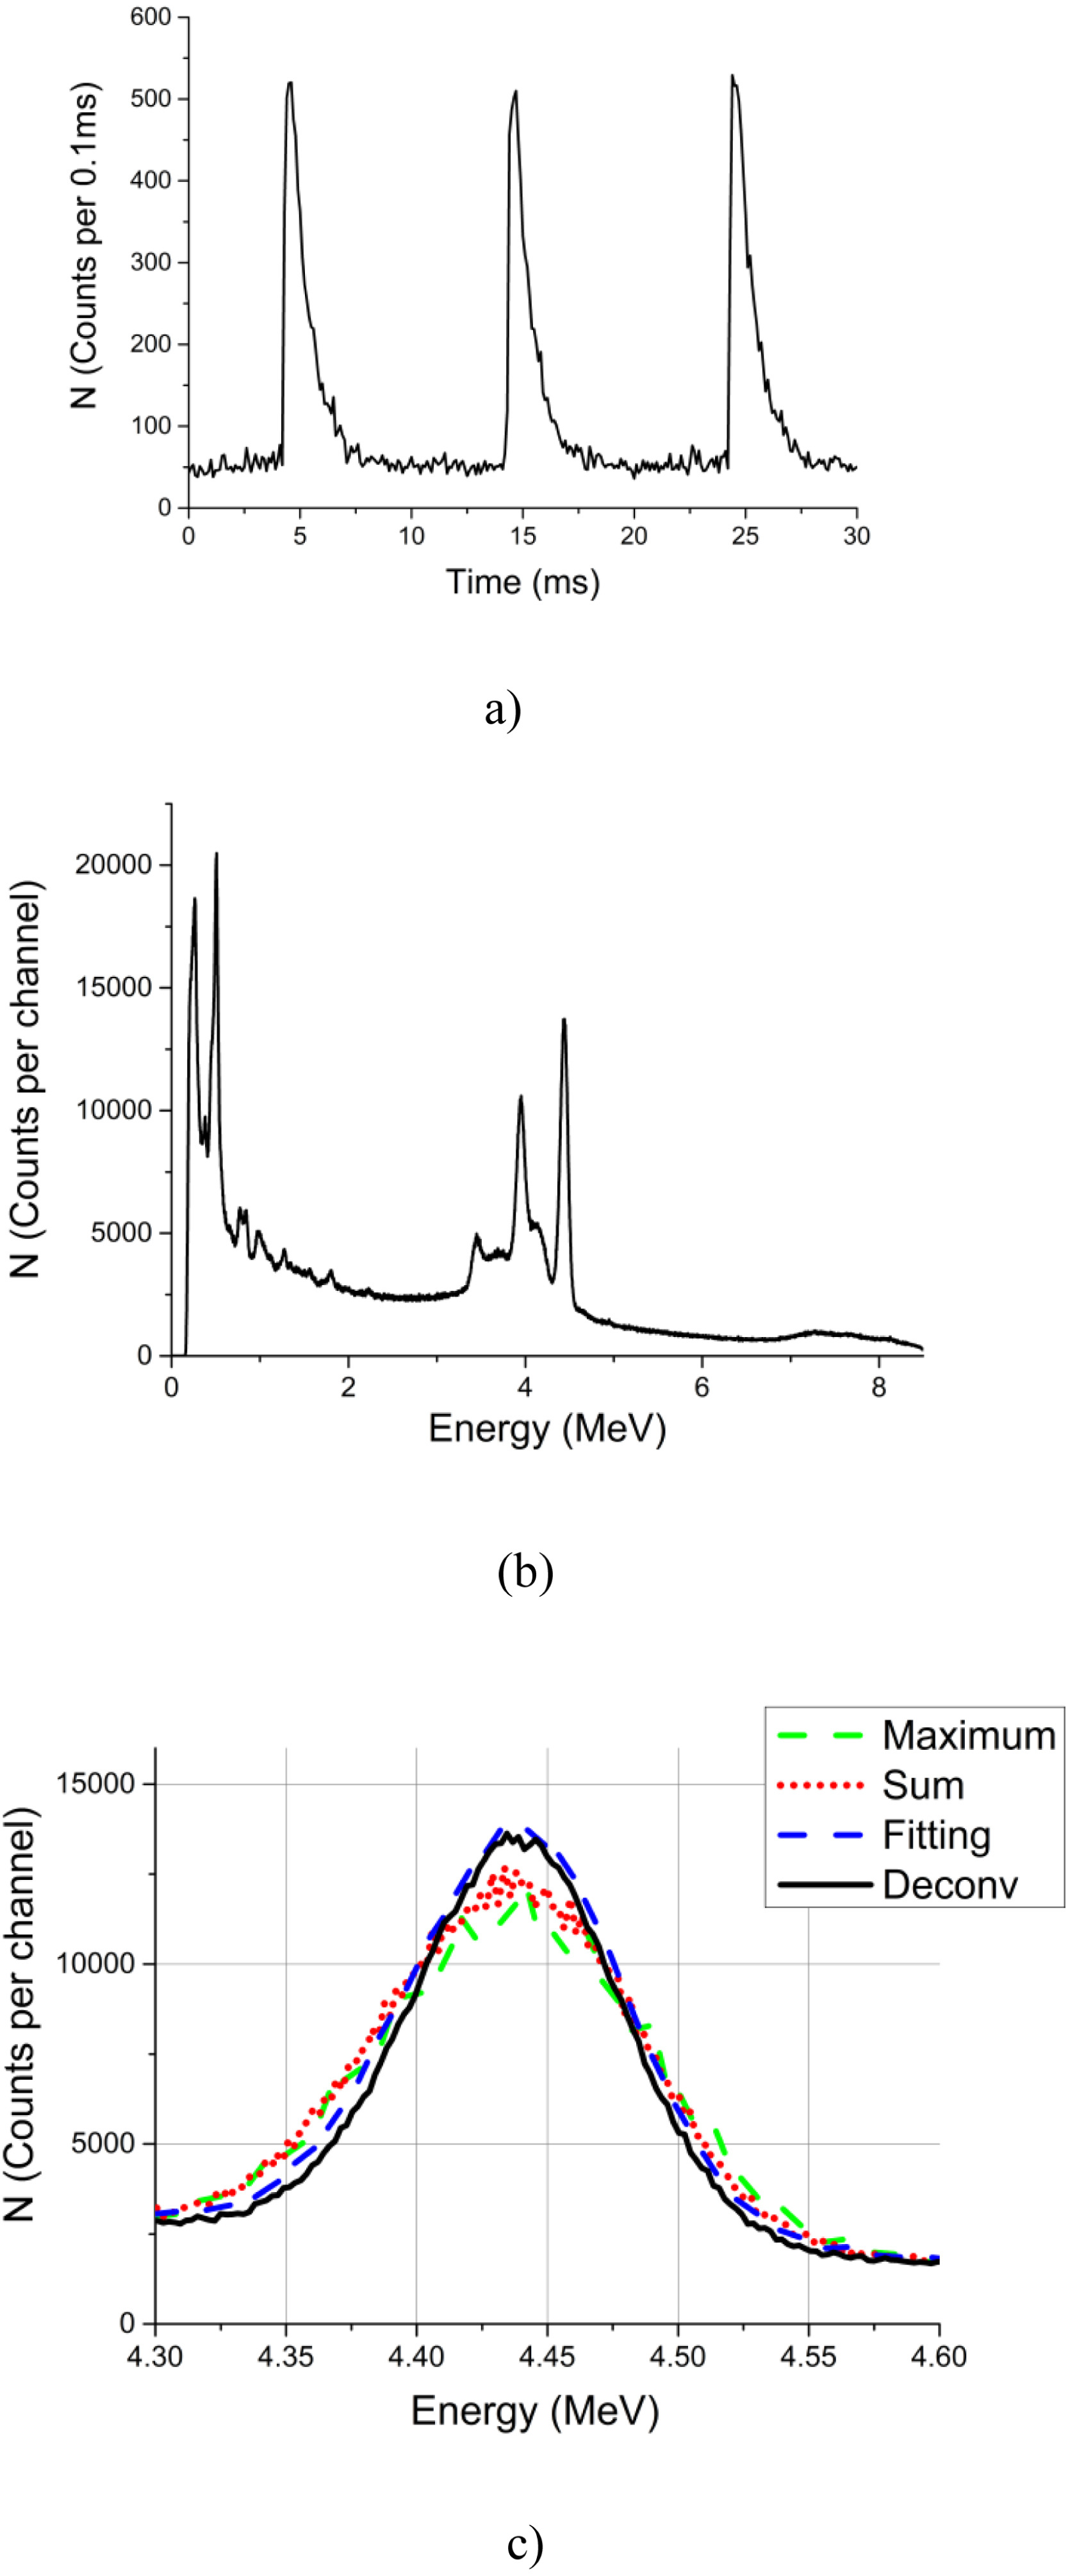
\includegraphics[width=0.51\linewidth]{processingCycloSignal} }
  \caption{ Результаты обработки сигнала, полученного в ходе измерений на циклотронне. a --- зависимость нагрузки детектора от времени (использовалась обработка методом фиттинга с коррекцией неразрешенных событий); b --- спектры гамма-излучения, полученные после обработки сигнала методом фиттинга; с --- cпектры гамма-излучения, полученные разными методами (построены вблизи пика 4.4~МэВ).~\cite{Khilkevitch2020} }
  \label{fig:processingCycloSignal}
\end{figure}

Результаты измерений представлены на рисунке~\ref{fig:processingCycloSignal}. Полная ширина на полувысоте (FWHM) пика 4.44~МэВ, полученная после обработки сигнала при максимальной нагрузке различными методами, представлена в таблице~\ref{tab:processingCycloSignal}. Видно что методы фиттинга и деконволюции имеют лучшее разрешение. Следует отметить, что линия 4.44~МэВ от реакции ${}^9Be(\alpha,n\gamma){}^{12}C$ уширена за счет эффекта Доплера. Доплеровская ширина линии для толстой бериллиевой мишени и пучка альфа-частиц с энергией 6~МэВ, ускоренного циклотроном, составляет примерно 51~кэВ.

\begin{table} [htbp]
    \centering
    \begin{threeparttable}
      \caption{ Полуширина пика с энергией 4.44~МэВ, полученная после обработки сигналов с использованием различных алгоритмов.~\cite{Khilkevitch2020} }
        \label{tab:processingCycloSignal}
        \begin{tabular}{| p{4cm} | p{6cm} | p{6cm} | }
            \hline
            Алгоритм   & Ширина линии, МэВ & \makecell{ Ошибка определения \\ ширины линии, МэВ } \\
            \hline
            По максимуму & 0.138 & 0.0019 \\
            Сумма &	0.135 &	0.0016\\
          Деконволюция &	0.093 &	0.0012 \\
          Фиттинг &	0.098 &	0.0012 \\
            \hline
        \end{tabular}
    \end{threeparttable}
\end{table}

С учетом эффекта Доплера рассчитанное энергетическое разрешение для линии 662~кэВ составило примерно 4.5\%. Однако следует отметить, что при таких нагрузках становится существенным эффект насыщения ФЭУ.

% ----------------------------------------------------------

\FloatBarrier
